% Options for packages loaded elsewhere
\PassOptionsToPackage{unicode}{hyperref}
\PassOptionsToPackage{hyphens}{url}
\PassOptionsToPackage{dvipsnames,svgnames,x11names}{xcolor}
%
\documentclass[
  12pt,
]{article}

\usepackage{amsmath,amssymb}
\usepackage{setspace}
\usepackage{iftex}
\ifPDFTeX
  \usepackage[T1]{fontenc}
  \usepackage[utf8]{inputenc}
  \usepackage{textcomp} % provide euro and other symbols
\else % if luatex or xetex
  \usepackage{unicode-math}
  \defaultfontfeatures{Scale=MatchLowercase}
  \defaultfontfeatures[\rmfamily]{Ligatures=TeX,Scale=1}
\fi
\usepackage{lmodern}
\ifPDFTeX\else  
    % xetex/luatex font selection
  \setmainfont[]{Times New Roman}
\fi
% Use upquote if available, for straight quotes in verbatim environments
\IfFileExists{upquote.sty}{\usepackage{upquote}}{}
\IfFileExists{microtype.sty}{% use microtype if available
  \usepackage[]{microtype}
  \UseMicrotypeSet[protrusion]{basicmath} % disable protrusion for tt fonts
}{}
\makeatletter
\@ifundefined{KOMAClassName}{% if non-KOMA class
  \IfFileExists{parskip.sty}{%
    \usepackage{parskip}
  }{% else
    \setlength{\parindent}{0pt}
    \setlength{\parskip}{6pt plus 2pt minus 1pt}}
}{% if KOMA class
  \KOMAoptions{parskip=half}}
\makeatother
\usepackage{xcolor}
\usepackage[margin=2cm]{geometry}
\setlength{\emergencystretch}{3em} % prevent overfull lines
\setcounter{secnumdepth}{5}
% Make \paragraph and \subparagraph free-standing
\ifx\paragraph\undefined\else
  \let\oldparagraph\paragraph
  \renewcommand{\paragraph}[1]{\oldparagraph{#1}\mbox{}}
\fi
\ifx\subparagraph\undefined\else
  \let\oldsubparagraph\subparagraph
  \renewcommand{\subparagraph}[1]{\oldsubparagraph{#1}\mbox{}}
\fi


\providecommand{\tightlist}{%
  \setlength{\itemsep}{0pt}\setlength{\parskip}{0pt}}\usepackage{longtable,booktabs,array}
\usepackage{calc} % for calculating minipage widths
% Correct order of tables after \paragraph or \subparagraph
\usepackage{etoolbox}
\makeatletter
\patchcmd\longtable{\par}{\if@noskipsec\mbox{}\fi\par}{}{}
\makeatother
% Allow footnotes in longtable head/foot
\IfFileExists{footnotehyper.sty}{\usepackage{footnotehyper}}{\usepackage{footnote}}
\makesavenoteenv{longtable}
\usepackage{graphicx}
\makeatletter
\def\maxwidth{\ifdim\Gin@nat@width>\linewidth\linewidth\else\Gin@nat@width\fi}
\def\maxheight{\ifdim\Gin@nat@height>\textheight\textheight\else\Gin@nat@height\fi}
\makeatother
% Scale images if necessary, so that they will not overflow the page
% margins by default, and it is still possible to overwrite the defaults
% using explicit options in \includegraphics[width, height, ...]{}
\setkeys{Gin}{width=\maxwidth,height=\maxheight,keepaspectratio}
% Set default figure placement to htbp
\makeatletter
\def\fps@figure{htbp}
\makeatother
% definitions for citeproc citations
\NewDocumentCommand\citeproctext{}{}
\NewDocumentCommand\citeproc{mm}{%
  \begingroup\def\citeproctext{#2}\cite{#1}\endgroup}
\makeatletter
 % allow citations to break across lines
 \let\@cite@ofmt\@firstofone
 % avoid brackets around text for \cite:
 \def\@biblabel#1{}
 \def\@cite#1#2{{#1\if@tempswa , #2\fi}}
\makeatother
\newlength{\cslhangindent}
\setlength{\cslhangindent}{1.5em}
\newlength{\csllabelwidth}
\setlength{\csllabelwidth}{3em}
\newenvironment{CSLReferences}[2] % #1 hanging-indent, #2 entry-spacing
 {\begin{list}{}{%
  \setlength{\itemindent}{0pt}
  \setlength{\leftmargin}{0pt}
  \setlength{\parsep}{0pt}
  % turn on hanging indent if param 1 is 1
  \ifodd #1
   \setlength{\leftmargin}{\cslhangindent}
   \setlength{\itemindent}{-1\cslhangindent}
  \fi
  % set entry spacing
  \setlength{\itemsep}{#2\baselineskip}}}
 {\end{list}}
\usepackage{calc}
\newcommand{\CSLBlock}[1]{\hfill\break\parbox[t]{\linewidth}{\strut\ignorespaces#1\strut}}
\newcommand{\CSLLeftMargin}[1]{\parbox[t]{\csllabelwidth}{\strut#1\strut}}
\newcommand{\CSLRightInline}[1]{\parbox[t]{\linewidth - \csllabelwidth}{\strut#1\strut}}
\newcommand{\CSLIndent}[1]{\hspace{\cslhangindent}#1}

\usepackage{booktabs}
\usepackage{longtable}
\usepackage{array}
\usepackage{multirow}
\usepackage{wrapfig}
\usepackage{float}
\usepackage{colortbl}
\usepackage{pdflscape}
\usepackage{tabu}
\usepackage{threeparttable}
\usepackage{threeparttablex}
\usepackage[normalem]{ulem}
\usepackage{makecell}
\usepackage{xcolor}
\usepackage[noblocks]{authblk}
\renewcommand*{\Authsep}{, }
\renewcommand*{\Authand}{, }
\renewcommand*{\Authands}{, }
\renewcommand\Affilfont{\small}
\makeatletter
\@ifpackageloaded{caption}{}{\usepackage{caption}}
\AtBeginDocument{%
\ifdefined\contentsname
  \renewcommand*\contentsname{Table of contents}
\else
  \newcommand\contentsname{Table of contents}
\fi
\ifdefined\listfigurename
  \renewcommand*\listfigurename{List of Figures}
\else
  \newcommand\listfigurename{List of Figures}
\fi
\ifdefined\listtablename
  \renewcommand*\listtablename{List of Tables}
\else
  \newcommand\listtablename{List of Tables}
\fi
\ifdefined\figurename
  \renewcommand*\figurename{Figure}
\else
  \newcommand\figurename{Figure}
\fi
\ifdefined\tablename
  \renewcommand*\tablename{Table}
\else
  \newcommand\tablename{Table}
\fi
}
\@ifpackageloaded{float}{}{\usepackage{float}}
\floatstyle{ruled}
\@ifundefined{c@chapter}{\newfloat{codelisting}{h}{lop}}{\newfloat{codelisting}{h}{lop}[chapter]}
\floatname{codelisting}{Listing}
\newcommand*\listoflistings{\listof{codelisting}{List of Listings}}
\makeatother
\makeatletter
\makeatother
\makeatletter
\@ifpackageloaded{caption}{}{\usepackage{caption}}
\@ifpackageloaded{subcaption}{}{\usepackage{subcaption}}
\makeatother
\ifLuaTeX
  \usepackage{selnolig}  % disable illegal ligatures
\fi
\usepackage{bookmark}

\IfFileExists{xurl.sty}{\usepackage{xurl}}{} % add URL line breaks if available
\urlstyle{same} % disable monospaced font for URLs
\hypersetup{
  pdftitle={Perceptions of Inequality and Meritocracy: Their Interplay in Shaping Preferences for Market Justice in Chile (2016-2023)},
  pdfauthor={Equipo EDUMER},
  colorlinks=true,
  linkcolor={blue},
  filecolor={Maroon},
  citecolor={Blue},
  urlcolor={Blue},
  pdfcreator={LaTeX via pandoc}}

\title{Perceptions of Inequality and Meritocracy: Their Interplay in
Shaping Preferences for Market Justice in Chile (2016-2023)}
\author{ }


\date{}
\begin{document}
\maketitle
\begin{abstract}
Several countries have experienced a shift toward the privatization and
commodification of public goods, welfare policies, and social services.
In Latin America, Chile stands out as a paradigmatic case where this
trend has led to the extensive marketization of essential services. From
a moral economy perspective, the extent to which individuals consider it
fair for access to such services to depend on market criteria has been
conceptualized as market justice preferences. This study investigates
the relationship between perceptions of economic inequality,
meritocratic beliefs, and market justice preferences in Chile between
2016 and 2023. Using six waves of panel data from the Chilean
Longitudinal Social Survey -- ELSOC (\(N_{observations}\) = 8,643;
\(N_{individuals}\) = 1,687), the analysis examines how subjective
assessments of inequality shape attitudes toward the role of merit in
access to key social services such as healthcare, education, and
pensions. The findings show that greater perceived inequality is
associated with lower market justice preferences. However, individuals
who believe that effort is rewarded are more likely to legitimize
existing disparities. In contrast, the perception that talent is
rewarded shows a negative effect on market justice preferences; an
effect that intensifies as perceived inequality increases over time. The
study also considers the influence of major social movements during this
period, which appear to have reshaped public discourse on justice and
fairness. These findings contribute to a deeper understanding of how
distributive beliefs evolve in contexts marked by persistent inequality
and entrenched neoliberal frameworks \newline \textbf{Keywords}:
Inequality perception, meritocracy, commodification, Chile, public
preferences
\end{abstract}

\setstretch{1.15}
\section{Introduction}\label{introduction}

Since 1980, economic inequality and wealth concentration have
dramatically increased worldwide, becoming one of the main challenges
for the social sciences. Globally, in 2021, less than 50\% of the world
population owned only 2\% of the wealth, while the richest 10\%
concentrated 76\%. Futhermore, the wealthiest 1\% captured nearly 38\%
of total assets (\citeproc{ref-chancel_world_2022}{Chancel et al.,
2022}). This context of economic disparity has sparked renewed interest
in studying not only the objective aspects of inequality, such as income
and access to resources, but also its subjective dimensions, including
perceptions, beliefs, and associated attitudes
(\citeproc{ref-janmaat_subjective_2013}{Janmaat, 2013}). Such dimensions
are deemed as key to understand the delegitimation of political
institutions that economic inequality can elicit
(\citeproc{ref-castillo_perception_2022}{Castillo et al., 2022}).
Therefore, understanding how people perceive inequality is crucial, as
these perceptions can influence how societies comprehend and justify (or
not) inequality in the distribution of goods and services, as well as
their capacity to funnel political discontent and eventually opposition
to the current economic distribution.

The justification of economic inequality is a topic with a long
tradition in sociology, with seminal works such as the ones from Kluegel
(\citeproc{ref-kluegel_social_1995a}{1995};
\citeproc{ref-kluegel_beliefs_1986}{1986}) and Lane
(\citeproc{ref-lane_political_1962}{1962},
\citeproc{ref-lane_market_1986}{1986}). Lane's main aim was to ``help
explain the tenacious hold of market capitalism on the public mind''
(\citeproc{ref-lane_market_1986}{1986, p. 384}), proposing the
distinction between market and political justice. Whereas political
justice refer to government actions aligned with justice principles such
equality or need, market justice involves the allocation linked to
earned desserts, particularly through individual contributions based on
individual merit. Part of this agenda has focused on analyzing the
extent to which individuals consider as just to get better access to
social services (such as pensions, health and education) based on
payment capacity (\citeproc{ref-busemeyer_skills_2014}{Busemeyer, 2014};
\citeproc{ref-castillo_socialization_2024}{Castillo et al., 2024};
\citeproc{ref-immergut_it_2020}{Immergut \& Schneider, 2020};
\citeproc{ref-koos_moral_2019}{Koos \& Sachweh, 2019};
\citeproc{ref-lindh_public_2015}{Lindh, 2015};
\citeproc{ref-lindh_bringing_2023}{Lindh \& McCall, 2023}), usually
under the label of market justice preferences. Although these services
can be considered fundamental rights of citizenship, existing evidence
indicates that a substantial share of the population legitimizes
inequality in these domains, and that such preferences are shaped by
individuals' socioeconomic characteristics as well as the broader
contextual features of their countries
(\citeproc{ref-busemeyer_skills_2014}{Busemeyer, 2014};
\citeproc{ref-koos_moral_2019}{Koos \& Sachweh, 2019};
\citeproc{ref-lindh_public_2015}{Lindh, 2015}). Within this framework,
we argue that there are two relevant factors that are usually sidelined
in this literature and that are key to understand market justice
preferences: the perception of economic inequality and the perception of
meritocracy.

The perception of economic inequality can be understood as an
individual's subjective assessment of how resources are allocated among
members of a given society (\citeproc{ref-akyelken_urban_2020}{Akyelken,
2020}). Regardless of their measurement, various studies have shown that
this perception often underestimates the gap between the rich and the
poor, revealing inconsistencies between objective and subjective aspects
of inequality (\citeproc{ref-trump_income_2018}{Trump, 2018}). Moreover,
there is consistent evidence that perceived inequality, even under
control of objective inequality, could have implications for attitudes
toward the distribution of goods and services
(\citeproc{ref-castillo_perception_2022}{Castillo et al., 2022};
\citeproc{ref-schroder_income_2017}{Schröder, 2017}), redistributive
preferences, justification of inequality, and legitimacy of the economic
system (\citeproc{ref-castillo_perception_2022}{Castillo et al., 2022};
\citeproc{ref-garcia-sanchez_attitudes_2020}{García-Sánchez et al.,
2020}, \citeproc{ref-garcia-sanchez_perceptions_2018}{2018}). From this
perspective, in this paper we argue that perceptions of economic
inequality would play a relevant role for understanding market justice
preferences, as a lower perceived inequality could reinforce the idea
that the differences in access to social services could be justified ---
a link that becomes harder to hold when high inequality is perceived.

Along with perception of inequality, a second focus of this paper is the
perception of meritocracy. Meritocracy posits that inequality can be
legitimized through distributive criteria such as effort and talent
(\citeproc{ref-davis_principles_2001}{Davis \& Moore, 2001};
\citeproc{ref-young_rise_1962}{Young, 1962}). Previous studies have
shown that those with stronger meritocratic perceptions tend to justify
larger inequality, as economic differences are legitimized by being
attributed to individual achievements
(\citeproc{ref-batruch_belief_2023}{Batruch et al., 2023};
\citeproc{ref-mijs_paradox_2021}{Mijs, 2021};
\citeproc{ref-wilson_role_2003}{Wilson, 2003}). We argue that in
contexts where the distribution of goods and services is predominantly
governed by market logics, as in the chilean case
(\citeproc{ref-boccardo_30_2020}{Boccardo, 2020};
\citeproc{ref-madariaga_three_2020}{Madariaga, 2020}), meritocratic
perceptions could play a role in the preferences of market justice.

The primary objective of this study is to analyze the interplay between
perceptions of inequality and meritocracy and their joint influence on
preferences for market justice along time in Chile using the panel
survey ELSOC (Social Chilean Longitudinal Study, 2016-2023).
Furthermore, we explore how political and social contingencies---such as
the 2019 and 2022 social movements---might have moderated these
relationships by prompting more critical reflection on the
commodification of social services (\citeproc{ref-somma_no_2021}{Somma
et al., 2021}). Recognizing the temporal dimension in shaping
preferences is essential, given that historical and contextual factors
that could challenge or reaffirm the way in which individuals perceive
inequality and meritocracy, resulting in changes in market justice
preferences.

\section{Market justice preferences}\label{market-justice-preferences}

Conceptually, \emph{market justice} has been discussed in the literature
as a normative principle that legitimates the distribution of economic
rewards based on individual merit. It is possible to trace the concept
to the understanding of Lane (\citeproc{ref-lane_market_1986}{1986}),
who makes a contrast between market justice and political justice. The
author defines market justice as a system of ``earned deserts'', whereby
individuals are seen as deserving of a determined distributive outcome
due to their effort and skills. In contrast, political justice
emphasizes principles of equality and need, which are often represented
by the welfare state action through social policies. An important remark
is that the principles of market justice rely on the assumption that
markets are neutral and self-regulating arenas, where individuals are
treated fairly because they face the same formal rules of engagement and
procedures (\citeproc{ref-lane_market_1986}{Lane, 1986}). Consequently,
the legitimacy of market justice stems from the assumption that
inequalities are not only inevitable but fair---so long as the rules are
transparent and opportunities are open. In this way, market justice
provides a moral justification for inequality by framing it as a
necessary outcome of individual responsibility
(\citeproc{ref-kluegel_legitimation_1999}{Kluegel et al., 1999};
\citeproc{ref-lindh_public_2015}{Lindh, 2015}).

Empirical studies have shown different strategies for the study of
market justice preferences. A common approach in the literature is to
gauge attitudes toward the legitimacy of inequality in specific domains,
especially when linked to income differences. This can be traced to the
seminal work of Kluegel and Smith
(\citeproc{ref-kluegel_beliefs_1981}{1981}) who assessed the normative
foundations that explain public support for economic inequality. Over
time, this approach has been extended beyond income to include other
market-mediated outcomes, such as education, healthcare, and/or
pensions. For example, Von Dem Knesebeck et al.
(\citeproc{ref-vondemknesebeck_are_2016}{2016}) and Immergut and
Schneider (\citeproc{ref-immergut_it_2020}{2020}) examine whether
citizens consider it fair that individuals with higher incomes can
access better healthcare, while Lee and Stacey
(\citeproc{ref-lee_fairness_2023}{2023}) apply a similar method in the
context of education in Australia. These studies usually rely on survey
items asking respondents to evaluate the fairness of income-based access
to welfare and social services(\citeproc{ref-lindh_public_2015}{Lindh,
2015}; \citeproc{ref-svallfors_political_2007}{Svallfors, 2007}). More
recently, Castillo et al.
(\citeproc{ref-castillo_socialization_2024}{2024}) introduced a
single-item composite measure of market justice to assess student
attitudes toward income-based access to education, healthcare, and
pensions in Chile. Such empirical strategies aim to capture the extent
to which individuals accept inequality when framed as a reflection of
market outcomes.

The study of market justice preferences has increasingly focused on how
they are shaped by individuals' socioeconomic position, normative
beliefs, and the institutional context in which they are embedded
(\citeproc{ref-pierson_when_1993}{Pierson, 1993}). Across the
literature, there is empirical evidence suggesting that individuals in
more advantaged socioeconomic positions---those with higher occupational
class, income, and education---are more likely to support market justice
principles (\citeproc{ref-koos_moral_2019}{Koos \& Sachweh, 2019};
\citeproc{ref-lindh_public_2015}{Lindh, 2015};
\citeproc{ref-svallfors_political_2007}{Svallfors, 2007}). This tendency
reflects not only material self-interest but also a broader moral
economy, in which winners of the market system internalize
justifications for the status quo. At the same time, political ideology
also plays a role ---such as economically conservative values --- where
right-wing individuals show higher support for meritocracy and more
skepticism towards redistribution. This is particularly salient in
countries with more restricted public provision of social services. For
example, in cases such as Chile
(\citeproc{ref-castillo_socialization_2024}{Castillo et al., 2024}) and
Australia(\citeproc{ref-lee_fairness_2023}{Lee \& Stacey, 2023}) the
evidence suggests that right-wing individuals are more supportive of
market-based distribution of welfare. Regarding contextual factors, in
liberal welfare regimes like those of the United States or the United
Kingdom, market justice preferences are more widespread, while in
coordinated or social-democratic regimes---such as Sweden or
Germany---citizens are generally more critical of market-based
inequalities (\citeproc{ref-immergut_it_2020}{Immergut \& Schneider,
2020}; \citeproc{ref-lindh_public_2015}{Lindh, 2015}).

\section{Perceptions of inequality and
meritocracy}\label{perceptions-of-inequality-and-meritocracy}

\emph{The perception of economic inequality}

Perceptions of inequality refer to individuals' subjective evaluations
of the extent, causes, and consequences of income and wealth disparities
(\citeproc{ref-akyelken_urban_2020}{Akyelken, 2020}). Unlike objective
measures such as the Gini index, perceived inequality captures how
individuals make sense of distributive hierarchies in their everyday
lives, shaped by reference groups, social comparisons, and information
environments (\citeproc{ref-garcia-castro_perceiving_2020}{García-Castro
et al., 2020}; \citeproc{ref-gimpelson_misperceiving_2018}{Gimpelson \&
Treisman, 2018}; \citeproc{ref-mijs_stratified_2016}{Mijs, 2016a}).
Scholars have proposed multiple dimensions of perceived inequality,
including its magnitude (how significant are the gaps), vertical
structure (between which groups), the trend over time (increasing or
decreasing), and legitimacy (whether it is just or not)
(\citeproc{ref-engelhardt_what_2018}{Engelhardt \& Wagener, 2018};
\citeproc{ref-garcia-sanchez_vicious_2019}{García-Sánchez et al.,
2019}). These dimensions encompass both cognitive and normative aspects
of perceptions of inequality and can vary across societies and social
groups, depending on exposure, ideology, and personal experience
(\citeproc{ref-castillo_perception_2022}{Castillo et al., 2022};
\citeproc{ref-garcia-sanchez_perceptions_2018}{García-Sánchez et al.,
2018}).

Perceptions of inequality have been associated with a range of
distributive attitudes (\citeproc{ref-castillo_perception_2022}{Castillo
et al., 2022}; \citeproc{ref-garcia-sanchez_vicious_2019}{García-Sánchez
et al., 2019}; \citeproc{ref-mccall_exposure_2017}{McCall et al., 2017};
\citeproc{ref-trump_income_2018}{Trump, 2018}). Research indicates that
perceptions of inequality influence redistributive preferences to a
greater extent than objective or actual economic inequality
(\citeproc{ref-Castillo2011}{Castillo, 2011};
\citeproc{ref-gimpelson_misperceiving_2018}{Gimpelson \& Treisman,
2018}). Lower perceived inequality can reinforce support for
market-based distributive arrangements
(\citeproc{ref-kuhn_eye_2011}{Kuhn, 2011}). In contrast, when inequality
is perceived as excessive, individuals could question the legitimacy of
market justice and become more supportive of redistributive policies
(\citeproc{ref-garcia-sanchez_vicious_2019}{García-Sánchez et al.,
2019}).

Assessing the perception of inequality in empirical research is an
ongoing challenge. Specifically in survey research, the assessment of
perceived inequality through Likert-type items such as ``income
differences are too large'' have been questioned as they captures
general concern or discomfort rather than a specific perception
(\citeproc{ref-Castillo2011}{Castillo, 2011};
\citeproc{ref-garcia-sanchez_vicious_2019}{García-Sánchez et al.,
2019}). As a result, the conceptual clarity between perceived inequality
and inequality aversion remains blurred in many empirical studies. To
address this limitation, recent work has emphasized the need to
distinguish between absolute and comparative measures, as well as
between ideal and perceived estimates of economic gaps
(\citeproc{ref-auspurg_why_2017}{Auspurg et al., 2017};
\citeproc{ref-garcia-sanchez_creencias_2022}{García-Sánchez \& De
Carvalho, 2022}). Through asking perceived salaries for occupations in
the extremes of the status continuum (such as a CEO and a manual
worker), an indirect measure of perceived inequality is built by the
ratio of the high and the low status occupation. This type of measure
provides a concrete frame that respondents can relate to more easily
than abstract questions about national income distribution
(\citeproc{ref-castillo_percepcion_2019}{Castillo et al., 2012};
\citeproc{ref-easterbrook_social_2021}{Easterbrook, 2021};
\citeproc{ref-willis_legitimacy_2015}{Willis et al., 2015}). Evidence to
date shows that perceived wage gaps are strong predictors of political
attitudes (\citeproc{ref-garcia-sanchez_perceptions_2018}{García-Sánchez
et al., 2018}; \citeproc{ref-pedersen_attitudes_2019}{Pedersen \& Mutz,
2019}), making them a valuable tool for understanding public responses
to economic disparities.

\emph{Perception of meritocracy}

Meritocracy constitutes a central ideological framework for legitimizing
various forms of social inequality
(\citeproc{ref-mijs_unfulfillable_2016}{Mijs, 2016b};
\citeproc{ref-wilson_role_2003}{Wilson, 2003}). Rooted in the belief
that rewards and social positions should be allocated based on
individual effort and talent, meritocracy operates both as a descriptive
account of how societies function and as a normative ideal of how they
ought to function. As originally conceptualized by Michael Young
(\citeproc{ref-young_rise_1962}{1962}), the term was intended as a
critique of a system in which merit-based stratification gives rise to a
new form of inequality. However, over time, meritocracy has come to be
widely endorsed as a fair and desirable principle of distribution,
particularly within liberal democracies and market-oriented societies
(\citeproc{ref-mijs_paradox_2021}{Mijs, 2021};
\citeproc{ref-sandel_tyranny_2020}{Sandel, 2020}).

From a sociological perspective, belief in meritocracy extends beyond a
cognitive judgment; it constitutes a moral lens through which
individuals interpret social and economic disparities
(\citeproc{ref-mijs_paradox_2021}{Mijs, 2021}). Individuals who believe
that success results from hard work and talent are more likely to regard
inequality as legitimate (\citeproc{ref-batruch_belief_2023}{Batruch et
al., 2023}; \citeproc{ref-castillo_percepcion_2019}{Castillo et al.,
2012}; \citeproc{ref-tejero-peregrina_perceived_2025}{Tejero-Peregrina
et al., 2025}). In contrast, when outcomes are attributed to luck,
social origin, or structural barriers, inequality is more often
perceived as unjust (\citeproc{ref-hauser_misperceptions_2017}{Hauser \&
Norton, 2017}; \citeproc{ref-reynolds_perceptions_2014}{Reynolds \&
Xian, 2014}). This distinction becomes especially salient in societies
marked by persistent structural inequality, where dominant narratives
emphasize personal responsibility while neglecting the role of
entrenched disadvantage.

Recent research has highlighted the importance of disentangling the
concept of ``meritocratic beliefs,'' particularly by distinguishing
between meritocratic preferences and meritocratic perceptions
(\citeproc{ref-castillo_multidimensional_2023}{Castillo et al., 2023}).
While preferences refer to normative ideals about how rewards should be
allocated (i.e., based on merit), perceptions refer to subjective
evaluations of how meritocracy actually operates in practice (i.e., how
rewards are allocated) (\citeproc{ref-janmaat_subjective_2013}{Janmaat,
2013}). This distinction allows for a more precise understanding of how
individuals make sense of inequality: people may endorse meritocracy
normatively while simultaneously recognizing its failure in practice. In
stratified societies, the gap between preferences and perceptions is
particularly evident, as individuals may continue to uphold the ideal of
meritocracy despite growing awareness of unequal opportunities
(\citeproc{ref-mijs_belief_2022}{Mijs et al., 2022}).

Within the domain of meritocratic perceptions
(\citeproc{ref-castillo_multidimensional_2023}{Castillo et al., 2023}),
we further distinguish between two core dimensions: effort-based and
talent-based perceptions. This distinction is analytically important, as
it captures different mechanisms through which individuals may justify
inequality (\citeproc{ref-reynolds_perceptions_2014}{Reynolds \& Xian,
2014}; \citeproc{ref-young_rise_1962}{Young, 1962}). Effort-based
perceptions emphasize hard work and perseverance as the key drivers of
success, aligning closely with cultural narratives of individual
responsibility and moral deservingness
(\citeproc{ref-dubet_repensar_2011}{Dubet, 2011}). In contrast,
talent-based perceptions emphasize innate ability and
intelligence---traits often regarded as less malleable and more
unequally distributed (\citeproc{ref-young_rise_1962}{Young, 1962}). We
argue that this latter dimension may shape attitudes differently, as
talent tends to be seen as a given attribute rather than the result of
personal effort.

Meritocratic perceptions function as a normative framework that
legitimizes unequal outcomes, particularly when access to social goods
is stratified by income or socioeconomic background. Prior studies have
consistently shown that individuals who perceive society as meritocratic
express lower support for redistribution
(\citeproc{ref-hoyt_mindsets_2023}{Hoyt et al., 2023};
\citeproc{ref-tejero-peregrina_perceived_2025}{Tejero-Peregrina et al.,
2025}), greater legitimization of class inequality
(\citeproc{ref-batruch_belief_2023}{Batruch et al., 2023}), increased
tolerance for inequality (\citeproc{ref-day_movin_2017}{Day \& Fiske,
2017}), and lower perceptions of income inequality itself
(\citeproc{ref-castillo_percepcion_2019}{Castillo et al., 2012}).
Regarding market justice preferences, prior studies in Chile have shown
that individuals who perceive higher levels of meritocracy tend to
express stronger support for unequal distributions that reflect market
outcomes in healthcare, education and pensions
(\citeproc{ref-castillo_socialization_2024}{Castillo et al., 2024}).
Taken together, and as Busemeyer et al.
(\citeproc{ref-busemeyer_positive_2021}{2021}) argues, meritocratic
narratives can operate as feedback mechanisms that shape public opinion
and individual well-being by framing welfare outcomes as either deserved
or undeserved. Such mechanism underscores the normative power of
meritocracy in stabilizing unequal systems by shaping political
attitudes and personal understandings of success and failure.

\subsection{The Chilean context}\label{the-chilean-context}

Chile offers an interesting case for examining how public attitudes
toward the distribution of social services evolve amid declining poverty
and persistently high income inequality within a residual welfare
framework (\citeproc{ref-ferre_welfare_2023}{Ferre, 2023}). Following
the neoliberal reforms of the 1980s introduced during the civil-military
dictatorship (1973-1989), the Chilean welfare state has become
increasingly reliant on private provision, with essential services often
commodified and largely reserved for those with sufficient purchasing
power (\citeproc{ref-boccardo_30_2020}{Boccardo, 2020};
\citeproc{ref-madariaga_three_2020}{Madariaga, 2020}). This model has
favored the affluent, while lower-income groups are left dependent on
limited and underfunded public alternatives. Research on social
stratification characterizes Chile as a society where mobility into
intermediate classes is feasible, but access to elite strata remains
largely restricted
(\citeproc{ref-lopez-roldan_comparative_2021}{López-Roldán \& Fachelli,
2021}; \citeproc{ref-torche_intergenerational_2014a}{Torche, 2014}).
While some indicators---such as education and occupation---suggest a
relatively fluid class structure, income mobility remains constrained
(\citeproc{ref-espinoza_movilidad_2014}{Espinoza \& Núñez, 2014}).

Despite steady economic expansion, Chile continues to rank among the
most unequal nations in the OECD, marked by a high Gini coefficient and
substantial wealth concentration at the top
(\citeproc{ref-flores_top_2020}{Flores et al., 2020}). In this context,
Chile experienced a wave of mass protests from October 2019 to March
2020. Initially led by high school students, the demonstrations quickly
gained momentum as broader segments of society mobilized around demands
for more equality of opportunities, particularly regarding precarious
access to welfare services. The political system interpreted this unrest
as a call to reform existing political institutions, with a special
focus on equalizing opportunities and providing more egalitarian access
to welfare by reducing reliance on out-of-pocket mechanisms
(\citeproc{ref-somma_no_2021}{Somma et al., 2021}).

\subsection{This study}\label{this-study}

Building upon the previous literature, this study proposes that
attitudes toward market justice are shaped by a dynamic interplay
between individuals' perceptions of economic inequality and their
perceptions of meritocracy. Specifically, we argue that both perceptions
independently and interactively influence the extent to which
individuals endorse market-based distributions of social goods and
services in Chile. To our knowledge, there are not studies so fay
analyzing such associations, let alone from a longitudinal perspective.

Firstly, and consistent with previous findings about research on
redistributive preferences
(\citeproc{ref-castillo_perception_2022}{Castillo et al., 2022}), we
expect that a higher perception of economic inequality will be
associated with lower market justice preferences. When individuals
perceive smaller income gaps, they are more likely to view market
mechanisms as fair and legitimate, reinforcing the acceptance of
outcomes based on competition and ability to pay. Conversely, a
heightened perception of inequality may erode confidence in market
fairness, weakening support for market-based distribution. This
relationship is particularly relevant in the context of Chile, where the
neoliberal economic model has been a dominant force in shaping public
attitudes toward inequality and justice
(\citeproc{ref-canalesceron_sujeto_2021}{Canales Cerón et al., 2021};
\citeproc{ref-mac-clure_justicia_2024}{Mac-Clure et al., 2024}).

Second, higher perceived meritocracy is expected to be positively
associated with market justice preferences. Individuals who believe that
effort and talent primarily determine success would be more likely to
justify unequal outcomes and endorse the notion that markets allocate
resources fairly according to individual merit
(\citeproc{ref-castillo_socialization_2024}{Castillo et al., 2024}).
This aligns with the idea that meritocratic perceptions serve as a moral
framework that legitimizes market-based inequalities, as individuals
perceive the system as just when they believe that rewards are based on
individual merit. This is particularly relevant in contexts where
neoliberal ideologies dominate, as they often emphasize individual
responsibility and competition as the basis for social order.

Third, we propose that perceptions of meritocracy and perceptions of
economic inequality interact in shaping market justice attitudes.
Specifically, we argue that the legitimizing effect of perceived
meritocracy on market justice preferences is moderated by perceived
economic inequality: when perceived inequality is low, the positive
association between meritocratic perceptions and market justice
preferences will be stronger. However, when perceived inequality is
high, this association will weaken, as greater awareness of large
economic gaps may challenge the view that outcomes are purely
merit-based.

Additionally, this study examines whether these relationships vary over
time, particularly in light of broader social and political
transformations. We are especially interested in whether changes in
individuals' perceptions of inequality and meritocracy are associated
with shifts in their market justice attitudes across different time
points. While we acknowledge the relevance of contextual events for
public opinion and political orientation
(\citeproc{ref-disipavlic_justification_2025}{Disi Pavlic et al.,
2025}), such as the 2019 political outburst or the subsequent
constitutional process in CHile, we are aware that identifying causal
associations lies outside the scope of this research. Instead, and from
an exploratory perspective, we focus on how intra-individual
trajectories in perceived inequality and merit shape evolving attitudes
toward the commodification of social services.

Based on these arguments, we propose the following hypotheses:

\(H1_{a} \; (\text{Between-person}):\) Individuals who perceive higher
levels of economic inequality will report lower support for market
justice preferences, on average, compared to those who perceive lower
levels of inequality.

\(H1_{b} \; (\text{Within-person}):\) Increases in an individual's
perception of economic inequality over time will be associated with
decreases in their support for market justice preferences.

\(H2_{a} \; (\text{Between-person}):\) Individuals who endorse stronger
meritocratic perceptions will report higher support for market justice
preferences, on average, compared to those with weaker meritocratic
perceptions

\(H2_{b} \; (\text{Within-person}):\) Increases in an individual's
meritocratic perceptions over time will be associated with increases in
their support for market justice preferences.

\(H3_{a} \; (\text{Between-person}):\) The positive association between
meritocratic perceptions and market justice preferences will be weaker
among individuals who perceive higher levels of economic inequality,
compared to those who perceive lower inequality.

\(H3_{b} \; (\text{Within-person}):\) The positive association between
meritocratic perceptions and market justice preferences will be weaker
at times when individuals perceive higher levels of inequality, relative
to times when they perceive lower inequality.

\(H4_{a} \; (\text{Growth moderation – Inequality}):\) The longitudinal
association between perceived economic inequality and market justice
preferences will strengthen over time, both within and between
individuals.

\(H4_{b} \; (\text{Growth moderation – Meritocracy}):\) The longitudinal
association between meritocratic perceptions and market justice
preferences will weaken over time, both within and between individuals.

\section{Data, Variables and Methods}\label{data-variables-and-methods}

\subsection{Data}\label{data}

This study draws on data from the Chilean Longitudinal Social Survey
(ELSOC), a nationally representative panel study of the urban adult
population in Chile, conducted annually between 2016 and 2023. Designed
to examine individuals' attitudes, emotions, and behaviors regarding
social conflict and cohesion, ELSOC employs a probabilistic, stratified,
clustered, and multistage sampling design covering both major urban
centers and smaller cities. The sampling frame was proportionally
stratified into six categories of urban population size (e.g., large and
small cities), followed by the random selection of households within
1,067 city blocks. The target population includes men and women aged 18
to 75 who are habitual residents of private dwellings.

The survey has been conducted every year since 2016, except in 2020,
when it was suspended due to the COVID-19 pandemic. This study uses six
waves: 2016, 2017, 2018, 2019, 2022, and 2023. The 2021 wave was
excluded because a reduced version of the questionnaire omitted key
variables of interest. Between waves 1 and 6, panel attrition reached
40\%, resulting in a final two-level sample comprising N = 8,643
observations nested within N = 1,687 individuals. Longitudinal weights
are applied to adjust for both the sampling design and potential biases
from systematic non-response. Further details on sampling, attrition,
and weighting procedures are available at
\url{https://coes.cl/encuesta-panel/}, and the dataset is publicly
accessible at \url{https://dataverse.harvard.edu/dataverse/elsoc}.

\subsection{Variables}\label{variables}

\textbf{Market justice preferences}: the dependent variable in this
study is preferences for market justice. This construct is
operationalized through three items that capture how strongly
individuals justify conditioning access to core services---healthcare,
pensions, and education--- basen on individual income. Specifically, the
justification of inequality in healthcare is assessed by the question:
``Is it fair in Chile that people with higher incomes can access better
healthcare than people with lower incomes?'' The same question is posed
for pensions and education. In all cases, respondents indicate their
level of agreement on a five-point Likert scale ranging from 1
(``strongly disagree'') to 5 (``strongly agree''). Additionally, we
include a composite measure of ``market justice preferences'',
calculated as the average of these three items (\(\alpha\) = 0.84). This
index ranges from 1 to 5, with higher values indicating stronger
preferences for market justice (see Table~\ref{tbl-summary1}).

\begin{longtable}[]{@{}
  >{\raggedright\arraybackslash}p{(\columnwidth - 6\tabcolsep) * \real{0.3367}}
  >{\raggedright\arraybackslash}p{(\columnwidth - 6\tabcolsep) * \real{0.3367}}
  >{\raggedright\arraybackslash}p{(\columnwidth - 6\tabcolsep) * \real{0.2143}}
  >{\raggedright\arraybackslash}p{(\columnwidth - 6\tabcolsep) * \real{0.1122}}@{}}
\caption{Dependent variables for the first wave
(2016)}\label{tbl-summary1}\tabularnewline
\toprule\noalign{}
\begin{minipage}[b]{\linewidth}\raggedright
Label
\end{minipage} & \begin{minipage}[b]{\linewidth}\raggedright
Stats / Values
\end{minipage} & \begin{minipage}[b]{\linewidth}\raggedright
Freqs (\% of Valid)
\end{minipage} & \begin{minipage}[b]{\linewidth}\raggedright
Valid
\end{minipage} \\
\midrule\noalign{}
\endfirsthead
\toprule\noalign{}
\begin{minipage}[b]{\linewidth}\raggedright
Label
\end{minipage} & \begin{minipage}[b]{\linewidth}\raggedright
Stats / Values
\end{minipage} & \begin{minipage}[b]{\linewidth}\raggedright
Freqs (\% of Valid)
\end{minipage} & \begin{minipage}[b]{\linewidth}\raggedright
Valid
\end{minipage} \\
\midrule\noalign{}
\endhead
\bottomrule\noalign{}
\endlastfoot
Health distributive justice &
\begin{minipage}[t]{\linewidth}\raggedright
1. Strongly desagree\\
2. Desagree\\
3. Neither agree nor desagre\\
4. Agree\\
5. Strongly agree\strut
\end{minipage} & \begin{minipage}[t]{\linewidth}\raggedright
558 (37.2\%)\\
729 (48.6\%)\\
63 ( 4.2\%)\\
133 ( 8.9\%)\\
18 ( 1.2\%)\strut
\end{minipage} & \begin{minipage}[t]{\linewidth}\raggedright
1501\\
(100.0\%)\strut
\end{minipage} \\
Pension distributive justice &
\begin{minipage}[t]{\linewidth}\raggedright
1. Strongly desagree\\
2. Desagree\\
3. Neither agree nor desagre\\
4. Agree\\
5. Strongly agree\strut
\end{minipage} & \begin{minipage}[t]{\linewidth}\raggedright
426 (28.4\%)\\
718 (47.8\%)\\
108 ( 7.2\%)\\
226 (15.1\%)\\
23 ( 1.5\%)\strut
\end{minipage} & \begin{minipage}[t]{\linewidth}\raggedright
1501\\
(100.0\%)\strut
\end{minipage} \\
Education distributive justice &
\begin{minipage}[t]{\linewidth}\raggedright
1. Strongly desagree\\
2. Desagree\\
3. Neither agree nor desagre\\
4. Agree\\
5. Strongly agree\strut
\end{minipage} & \begin{minipage}[t]{\linewidth}\raggedright
521 (34.7\%)\\
783 (52.2\%)\\
73 ( 4.9\%)\\
113 ( 7.5\%)\\
11 ( 0.7\%)\strut
\end{minipage} & \begin{minipage}[t]{\linewidth}\raggedright
1501\\
(100.0\%)\strut
\end{minipage} \\
Market justice preferences & \begin{minipage}[t]{\linewidth}\raggedright
Mean (sd) : 2 (0.8)\\
min \textless{} med \textless{} max:\\
1 \textless{} 2 \textless{} 5\\
IQR (CV) : 0.7 (0.4)\strut
\end{minipage} & 12 distinct values &
\begin{minipage}[t]{\linewidth}\raggedright
1501\\
(100.0\%)\strut
\end{minipage} \\
\end{longtable}

\textbf{Perception of economic inequality}: this variable is measured
through the perceived wage gap
(\citeproc{ref-castillo_cual_2009}{Castillo, 2009};
\citeproc{ref-gijsberts_thelegitimation_1999}{Gijsberts, 1999};
\citeproc{ref-hadler_why_2005}{Hadler, 2005}). This measure is derived
from the salary gap between the perceived salaries of jobs at opposite
ends of the occupational hierarchy. Specifically, it relies on the
division between the perceived salary of a large-company president and
that of an unskilled worker (\citeproc{ref-Castillo2011}{Castillo,
2011}). Higher values of this term indicate a greater perception of
economic inequality between occupations located at the extremes of the
status continuum. This measure includes a logarithmic term in order to
adjust income magnitudes (usually fewer cases with high income):

\[
\text{perceived wage gap} = \log_{10}\left(\frac{\text{perceived salary of a large-company president}}{\text{perceived salary of an unskilled worker}}\right)
\]

\textbf{Perception of Meritocracy}: this variable is operationalized
through two components, namely effort and talent
(\citeproc{ref-young_rise_1962}{Young, 1962}). The item used to gauge
effort is: ``In Chile, people are rewarded for their efforts,'' while
the item for talent is: ``In Chile, people are rewarded for their
intelligence and skills''. In both cases, respondents indicate their
level of agreement on a five-point Likert scale, ranging from 1
(``strongly disagree'') to 5 (``strongly agree'').

Table 2 shows the independent variables used, their response categories
and their frequencies.

\begin{longtable}[]{@{}
  >{\raggedright\arraybackslash}p{(\columnwidth - 6\tabcolsep) * \real{0.3774}}
  >{\raggedright\arraybackslash}p{(\columnwidth - 6\tabcolsep) * \real{0.3113}}
  >{\raggedright\arraybackslash}p{(\columnwidth - 6\tabcolsep) * \real{0.2075}}
  >{\raggedright\arraybackslash}p{(\columnwidth - 6\tabcolsep) * \real{0.1038}}@{}}
\caption{Independent variables ELSOC survey (descriptives for first wave
2016)}\label{tbl-summary2}\tabularnewline
\toprule\noalign{}
\begin{minipage}[b]{\linewidth}\raggedright
Label
\end{minipage} & \begin{minipage}[b]{\linewidth}\raggedright
Stats / Values
\end{minipage} & \begin{minipage}[b]{\linewidth}\raggedright
Freqs (\% of Valid)
\end{minipage} & \begin{minipage}[b]{\linewidth}\raggedright
Valid
\end{minipage} \\
\midrule\noalign{}
\endfirsthead
\toprule\noalign{}
\begin{minipage}[b]{\linewidth}\raggedright
Label
\end{minipage} & \begin{minipage}[b]{\linewidth}\raggedright
Stats / Values
\end{minipage} & \begin{minipage}[b]{\linewidth}\raggedright
Freqs (\% of Valid)
\end{minipage} & \begin{minipage}[b]{\linewidth}\raggedright
Valid
\end{minipage} \\
\midrule\noalign{}
\endhead
\bottomrule\noalign{}
\endlastfoot
Inequality gap perception & \begin{minipage}[t]{\linewidth}\raggedright
Mean (sd) : 3.7 (1.1)\\
min \textless{} med \textless{} max:\\
0.4 \textless{} 3.7 \textless{} 6.9\\
IQR (CV) : 1.6 (0.3)\strut
\end{minipage} & 296 distinct values &
\begin{minipage}[t]{\linewidth}\raggedright
1501\\
(100.0\%)\strut
\end{minipage} \\
People are rewarded for their efforts &
\begin{minipage}[t]{\linewidth}\raggedright
1. Strongly desagree\\
2. Desagree\\
3. Neither agree nor desagre\\
4. Agree\\
5. Strongly agree\strut
\end{minipage} & \begin{minipage}[t]{\linewidth}\raggedright
169 (11.3\%)\\
693 (46.2\%)\\
263 (17.5\%)\\
328 (21.9\%)\\
48 ( 3.2\%)\strut
\end{minipage} & \begin{minipage}[t]{\linewidth}\raggedright
1501\\
(100.0\%)\strut
\end{minipage} \\
People are rewarded for their intelligence &
\begin{minipage}[t]{\linewidth}\raggedright
1. Strongly desagree\\
2. Desagree\\
3. Neither agree nor desagre\\
4. Agree\\
5. Strongly agree\strut
\end{minipage} & \begin{minipage}[t]{\linewidth}\raggedright
134 ( 8.9\%)\\
617 (41.1\%)\\
294 (19.6\%)\\
401 (26.7\%)\\
55 ( 3.7\%)\strut
\end{minipage} & \begin{minipage}[t]{\linewidth}\raggedright
1501\\
(100.0\%)\strut
\end{minipage} \\
\end{longtable}

\emph{Controls}

Sociodemographic and attitudinal variables are included to control for
potential composition effects in the population. In terms of
sociodemographic characteristics, we incorporate per capita household
income quintile, educational level (1=Less than Universitary,
2=Universitary), age (in ranges), and sex (1=Male, 2=Female), which have
been previously shown to influence market justice preferences
significantly (\citeproc{ref-castillo_socialization_2024}{Castillo et
al., 2024}; \citeproc{ref-lindh_public_2015}{Lindh, 2015}). Regarding
attitudinal variables, we include political identification (1=Left,
2=Center, 3=Right, 4=No identification) and subjective social status
(measured through a scale from 1 to 10) as they may affect the
relationship between market justice preferences, perceptions of
inequality, and meritocracy
(\citeproc{ref-schneider_poverty_2015}{Schneider \& Castillo, 2015}).
Descriptive statistics for the control variables can be found in the
supplementary material.

\subsection{Methods}\label{methods}

Given the data's hierarchical structure, in which observations are
nested in survey waves, we employ longitudinal multilevel linear models
(\citeproc{ref-singer_applied_2009}{Singer \& Willett, 2009}). In a
panel-data framework, within-person effects capture how shifts in
individual-level variables across waves are associated with variations
in market justice preferences. By contrast, between-person effects focus
on differences among individuals, explaining how long-term (or average)
values relate to overall levels of market justice preferences.

To estimate within-person effects, we use group-mean centering, where
each respondent functions as the ``group'' (i.e., observations nested
within persons). Meanwhile, the between-person effects are derived from
each individual's average on these variables, calculated across the
waves of panel data.

All the analyses were conducted using R software and the \emph{lme4}
package (\citeproc{ref-bates_fitting_2015}{Bates et al., 2015}).

\section{Results}\label{results}

\subsection{Descriptive statistics}\label{descriptive-statistics}

Figure~\ref{fig-alluvial} shows the annual frequencies of market justice
preferences for healthcare, pensions, and education from 2016 to 2023.
Each year presents stacked percentage frequencies, and the flows between
them reflect opinion changes among the same individuals from one year to
the next, given that we are using panel data. For instance, of the
40.8\% who strongly disagreed with justifying inequality in healthcare
in 2019, around 24.3\% maintained that position in 2022, while the
remaining 16.5\% shifted toward other response categories---primarily
moving into disagreement rather than strong disagreement. Overall, more
than half of the respondents exhibit a high level of disagreement
(disagree + strongly disagree) with inequality in these three social
service areas over time. Despite this general pattern, recent waves show
a slight decrease in disagreement and a corresponding rise in support
for market-justice inequality. Specifically, in healthcare and
education, although disagreement remains substantial, agreement (agree +
strongly agree) increased from 7.4\% and 7.2\% in 2019 to 13.1\% and
14.2\% in 2023, respectively. This shift is most evident in pensions,
where the combined agree/strongly agree category grew by about 10
percentage points, from 16.9\% in 2016 to 28\% in 2023.

\begin{figure}[H]

\caption{\label{fig-alluvial}Change in the justification of inequality
in healthcare, pensions and education over time (2016-2023)}

\centering{

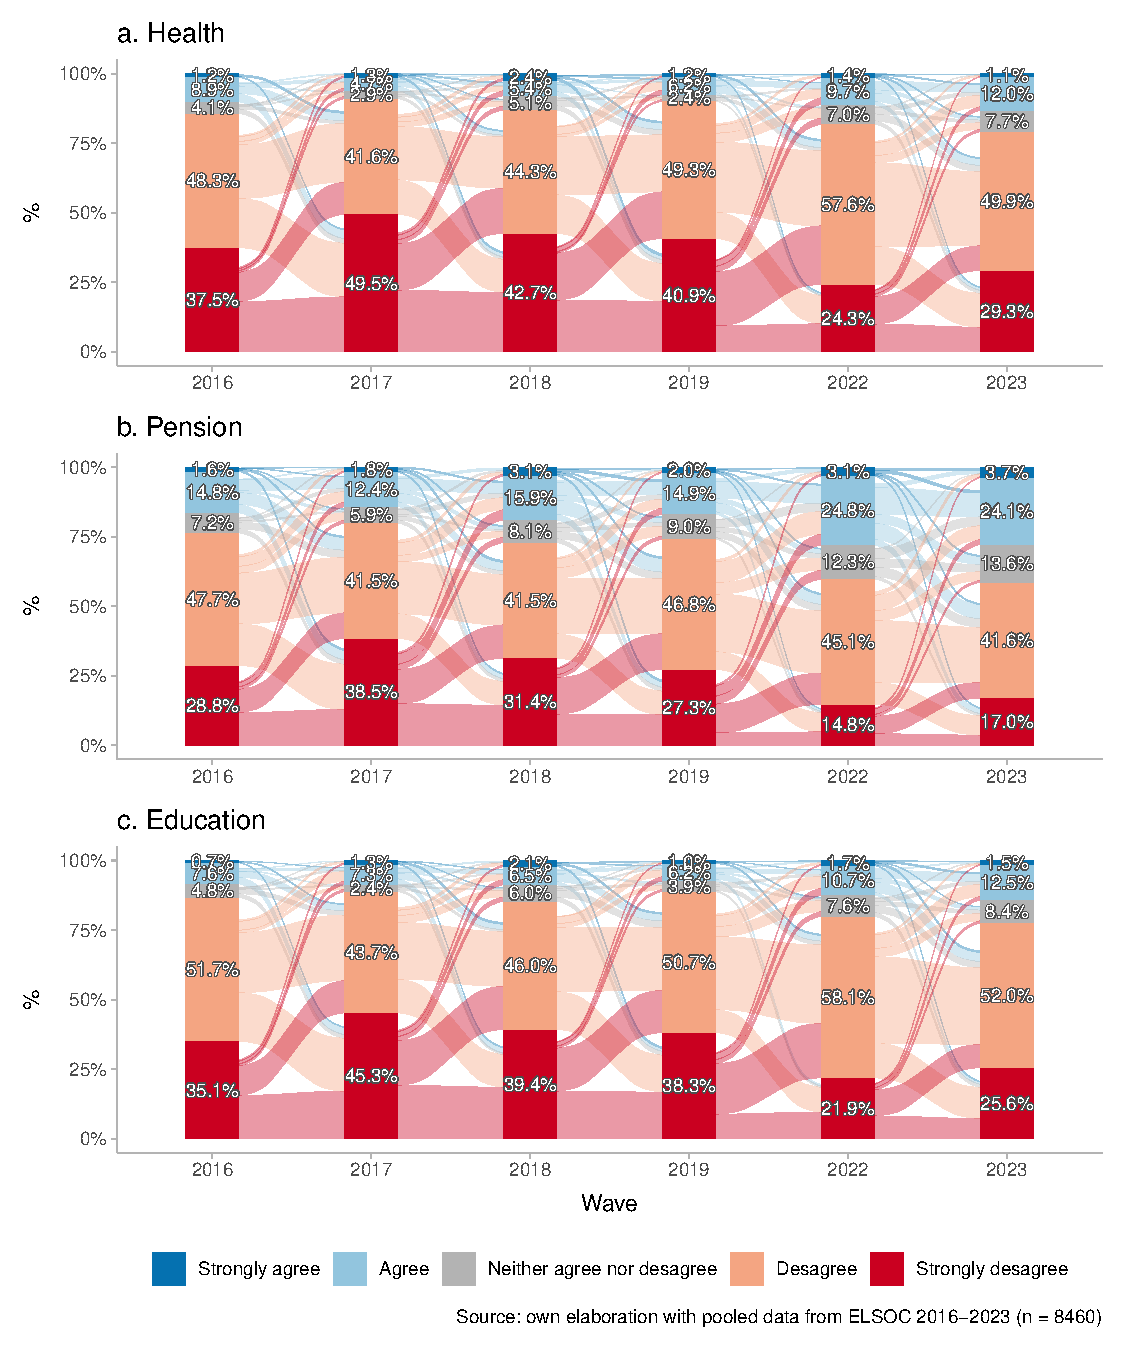
\includegraphics[width=1\textwidth,height=\textheight]{paper-blinded-resubmit_files/figure-pdf/fig-alluvial-1.pdf}

}

\end{figure}%

Regarding the main dependent and independent variables of this study,
Figure~\ref{fig-meanchange} depicts their standardized average values
across survey waves. The results show a notable upward trend in market
justice preferences, particularly in the most recent waves. Perceived
economic inequality exhibited the highest standardized mean in 2016;
however, this variable shows a general downward trajectory over time,
with a temporary increase in 2019, possibly reflecting the effects of
the social uprising that year. Interestingly, while perceptions of
inequality declined in the latest waves (2022--2023), market justice
preferences continued to rise. Meritocratic perceptions, in contrast,
remain relatively stable overall. Nevertheless, perceptions that
individuals are rewarded based on talent tend to be slightly higher than
those based on effort. Both meritocracy-related measures follow a
similar temporal pattern: an increase from 2016 to 2018, a decline
between 2019 and 2022---potentially associated with the social unrest
and the consequences of the COVID-19 pandemic---and a subsequent rise in
2023, returning to levels comparable to those observed in 2016.

\begin{figure}[H]

\caption{\label{fig-meanchange}Change in the standarized mean of market
justice preferences, economic inequality perception, and meritocracy
(2016-2023)}

\centering{

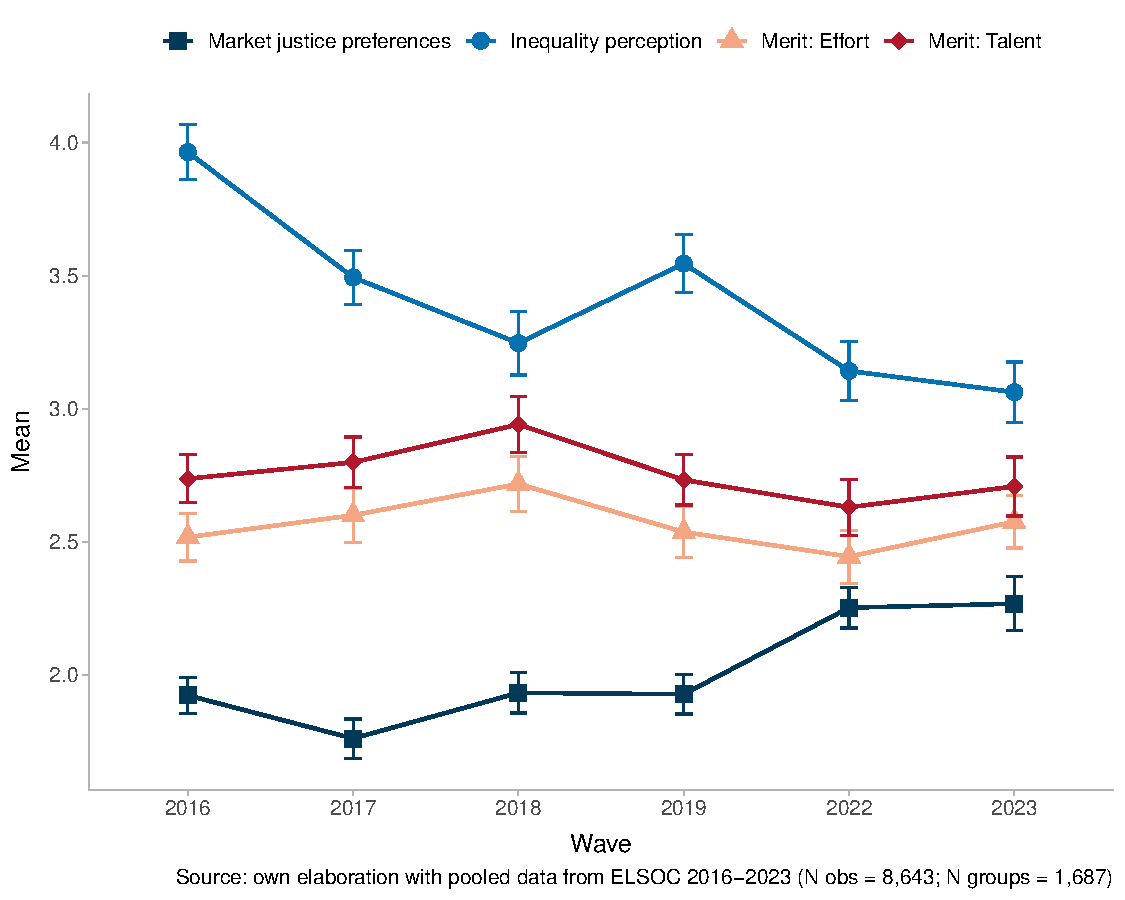
\includegraphics[width=1\textwidth,height=\textheight]{paper-blinded-resubmit_files/figure-pdf/fig-meanchange-1.pdf}

}

\end{figure}%

\subsection{Multilevel models}\label{multilevel-models}

Table~\ref{tbl-modelos} presents the results of the multilevel models
estimated for market justice preferences, examining both individuals
(within) and group-level (between) effects. The intraclass correlation
(\citeproc{ref-hoxMultilevelAnalysisTechniques2017a}{Hox et al., 2017})
from the empty model (see Supplementary Material), which decomposes the
variance of market justice preferences, is 0.31, indicating that
approximately 31\% of the variation is attributable to differences
between individuals. Complementary, 69\% of the variation corresponds to
within-individual differences over time.

\begin{table}

\caption{\label{tbl-modelos}Longitudinal multilevel models for market
justice preferences}

\centering{

\caption{}
\begin{center}
\scalebox{0.8}{
\begin{tabular}{l c c c c c c c}
\hline
 & Model 1 & Model 2 & Model 3 & Model 4 & Model 5 & Model 6 & Model 7 \\
\hline
Intercept                          & $1.938^{***}$  & $1.948^{***}$  & $1.965^{***}$  & $1.967^{***}$  & $1.974^{***}$  & $1.186^{***}$  & $1.250^{***}$  \\
                                   & $(0.023)$      & $(0.037)$      & $(0.037)$      & $(0.037)$      & $(0.087)$      & $(0.124)$      & $(0.144)$      \\
Wave (Ref.= 2016)                  &                &                &                &                &                &                &                \\
                                   &                &                &                &                &                &                &                \\
\quad Wave 2017                    & $-0.183^{***}$ &                &                &                &                &                &                \\
                                   & $(0.025)$      &                &                &                &                &                &                \\
\quad Wave 2018                    & $-0.009$       &                &                &                &                &                &                \\
                                   & $(0.025)$      &                &                &                &                &                &                \\
\quad Wave 2019                    & $-0.009$       &                &                &                &                &                &                \\
                                   & $(0.025)$      &                &                &                &                &                &                \\
\quad Wave 2022                    & $0.300^{***}$  &                &                &                &                &                &                \\
                                   & $(0.025)$      &                &                &                &                &                &                \\
\quad Wave 2023                    & $0.320^{***}$  &                &                &                &                &                &                \\
                                   & $(0.025)$      &                &                &                &                &                &                \\
Wave                               &                & $-0.088^{***}$ & $-0.095^{***}$ & $-0.096^{***}$ & $-0.096^{***}$ & $-0.096^{***}$ & $-0.096^{***}$ \\
                                   &                & $(0.020)$      & $(0.020)$      & $(0.020)$      & $(0.020)$      & $(0.020)$      & $(0.020)$      \\
Wave$^2$                           &                & $0.024^{***}$  & $0.024^{***}$  & $0.025^{***}$  & $0.025^{***}$  & $0.025^{***}$  & $0.025^{***}$  \\
                                   &                & $(0.003)$      & $(0.003)$      & $(0.003)$      & $(0.003)$      & $(0.003)$      & $(0.003)$      \\
Perception inequality (WE)         &                &                & $-0.027^{**}$  & $-0.025^{**}$  & $-0.025^{**}$  & $-0.025^{**}$  & $-0.025^{**}$  \\
                                   &                &                & $(0.009)$      & $(0.009)$      & $(0.009)$      & $(0.009)$      & $(0.009)$      \\
Merit: Effort (WE)                 &                &                &                & $0.070^{***}$  & $0.070^{***}$  & $0.070^{***}$  & $0.070^{***}$  \\
                                   &                &                &                & $(0.011)$      & $(0.011)$      & $(0.011)$      & $(0.011)$      \\
Merit: Talent (WE)                 &                &                &                & $-0.027^{*}$   & $-0.027^{*}$   & $-0.027^{*}$   & $-0.027^{*}$   \\
                                   &                &                &                & $(0.011)$      & $(0.011)$      & $(0.011)$      & $(0.011)$      \\
Perception inequality (BE)         &                &                &                &                & $-0.002$       & $0.043$        & $0.008$        \\
                                   &                &                &                &                & $(0.023)$      & $(0.023)$      & $(0.024)$      \\
Merit: Effort (BE)                 &                &                &                &                &                & $0.206^{***}$  & $0.191^{***}$  \\
                                   &                &                &                &                &                & $(0.041)$      & $(0.040)$      \\
Merit: Talent (BE)                 &                &                &                &                &                & $0.036$        & $0.021$        \\
                                   &                &                &                &                &                & $(0.040)$      & $(0.040)$      \\
\hline
Controls                           & No             & No             & No             & No             & No             & No             & Yes            \\
BIC                                & $32146.711$    & $31406.958$    & $31414.699$    & $31404.308$    & $31419.062$    & $31366.239$    & $31473.850$    \\
Numb. obs.                         & $8643$         & $8643$         & $8643$         & $8643$         & $8643$         & $8643$         & $8643$         \\
Num. groups: individuals           & $1687$         & $1687$         & $1687$         & $1687$         & $1687$         & $1687$         & $1687$         \\
Var: individuals (Intercept)       & $0.205$        & $0.370$        & $0.366$        & $0.363$        & $0.364$        & $0.336$        & $0.326$        \\
Var: Residual                      & $0.416$        & $0.345$        & $0.345$        & $0.343$        & $0.343$        & $0.343$        & $0.343$        \\
Var: individuals, wave             & $$             & $0.022$        & $0.021$        & $0.021$        & $0.021$        & $0.021$        & $0.021$        \\
Cov: individuals (Intercept), wave & $$             & $-0.061$       & $-0.060$       & $-0.059$       & $-0.059$       & $-0.058$       & $-0.059$       \\
\hline
\multicolumn{8}{l}{\scriptsize{Note: Cells contain regression coefficients with standard errors in parentheses. $^{***}p<0.001$; $^{**}p<0.01$; $^{*}p<0.05$.}}
\end{tabular}
}
\label{table:coefficients}
\end{center}

}

\end{table}%

According to Model 1, which includes the survey waves to capture
intertemporal variations in the dependent variable, there is a decrease
in 2017 (\(\beta\) = -0.183, \(p\) \textless{} .001) relative to 2016,
and similarly in 2018 (\(\beta\) = -0.009, \(p\) \textgreater{} .05) and
2019 (\(\beta\) = -0.009, \(p\) \textgreater{} .05), although the latter
effects are not statistically significant. In contrast, in the more
recent waves of 2022 and 2023, there is a statistically significant
increase in market justice preferences (\(\beta\) = 0.300, \(p\)
\textless{} .001; \(\beta\) = 0.320, \(p\) \textless{} .001), suggesting
a non-linear effect. To model this trajectory over time, Model 2
incorporates time (survey waves) as a continuous variable, along with
its quadratic term, representing the non-linear association initially
observed in Model 1. While the linear term (survey wave) shows a
negative association, reflecting an overall decline in market
preferences over time, the positive quadratic term indicates a reversal
of this pattern in the final measurement points.

Models 3 and 4 incorporate the within-group effects (WE) of the primary
independent variables, capturing how individual changes in these
variables over time shape the dependent variable. The results in Model 3
suggest that the within effect of perceived economic inequality is
negative and statistically significant (\(p\) \textless{} .001).
Specifically, each one-point increase in an individual's perception of
economic inequality between waves is associated with a 0.027 point
decrease in market justice preferences. Model 4 shows that meritocratic
perceptions operate in distinct directions. An upward shift in the
perception that effort is rewarded exerts a positive within effect
(\(\beta\) = 0.070, \(p\) \textless{} .001), while a parallel increase
in the perception that intelligence and ability are rewarded is likewise
associated with lower market-justice preferences (\(\beta\) = -0.027,
\(p\) \textless{} .05). Taken together, these results suggest that
people who increasingly perceive meritocracy based on effort tend to
have stronger preferences for market justice, and that the opposite is
true for those who increasingly perceive meritocracy based on talent.

When examining the between-group effects (BE) in Model 5 and 6, which
capture differences between individuals in the average of the main
variables, a similar pattern emerges. Individuals who perceive higher
levels of economic inequality tend to prefer less market justice
(\(\beta\) = -0.002, \(p\) \textgreater{} .05). However, this effect is
no longer statistically significant. In Model 6, the meritocratic
perception that effort is rewarded is positively associated with market
justice preferences (\(\beta\) = 0.206, \(p\) \textless{} .001), whereas
the perception that talent is rewarded shows a positive but
non-significant coefficient (\(\beta\) = 0.036, \(p\) \textgreater{}
.05).

Model 7 adds the control variables. The within- and between-effects of
the principal predictors retain both their direction and statistical
significance, confirming the robustness of the associations (see
Supplementary Material for effects of control variables).

\begin{table}

\caption{\label{tbl-interactions1}Interactions for meritocracy,
perceived economic inequality and market justice preferences}

\centering{

\caption{}
\begin{center}
\scalebox{0.8}{
\begin{tabular}{l c c c c}
\hline
 & Model 8 & Model 9 & Model 10 & Model 11 \\
\hline
Intercept                                                     & $1.328^{***}$ & $1.346^{***}$ & $1.956^{***}$  & $2.281^{***}$  \\
                                                              & $(0.143)$     & $(0.143)$     & $(0.350)$      & $(0.369)$      \\
Perception inequality (WE)                                    & $-0.037^{*}$  & $-0.036^{*}$  & $-0.040^{***}$ & $-0.040^{***}$ \\
                                                              & $(0.015)$     & $(0.015)$     & $(0.009)$      & $(0.009)$      \\
Merit: Effort (WE)                                            & $0.075^{***}$ & $0.085^{***}$ & $0.081^{***}$  & $0.081^{***}$  \\
                                                              & $(0.018)$     & $(0.012)$     & $(0.011)$      & $(0.011)$      \\
Merit: Talent (WE)                                            & $-0.021$      & $-0.017$      & $-0.026^{*}$   & $-0.026^{*}$   \\
                                                              & $(0.011)$     & $(0.016)$     & $(0.011)$      & $(0.011)$      \\
Perception inequality (BE)                                    & $-0.003$      & $-0.003$      & $-0.176$       & $-0.268^{**}$  \\
                                                              & $(0.023)$     & $(0.023)$     & $(0.096)$      & $(0.101)$      \\
Merit: Effort (BE)                                            & $0.180^{***}$ & $0.183^{***}$ & $-0.045$       & $0.191^{***}$  \\
                                                              & $(0.040)$     & $(0.040)$     & $(0.127)$      & $(0.041)$      \\
Merit: Talent (BE)                                            & $0.022$       & $0.018$       & $0.017$        & $-0.320^{*}$   \\
                                                              & $(0.039)$     & $(0.039)$     & $(0.041)$      & $(0.129)$      \\
Merit: Effort (WE) x Perception inequality (WE)               & $-0.014$      &               &                &                \\
                                                              & $(0.013)$     &               &                &                \\
Merit: Talent (WE) x Perception inequality (WE)               &               & $-0.032^{*}$  &                &                \\
                                                              &               & $(0.013)$     &                &                \\
Merit: Effort (BE) x Perception inequality (BE)               &               &               & $0.070$        &                \\
                                                              &               &               & $(0.036)$      &                \\
Merit: Talent (BE) x Perception inequality (BE)               &               &               &                & $0.099^{**}$   \\
                                                              &               &               &                & $(0.036)$      \\
\hline
Controls                                                      & Yes           & Yes           & Yes            & Yes            \\
BIC                                                           & $31201.714$   & $31254.484$   & $32281.698$    & $32277.809$    \\
Numb. obs.                                                    & $8643$        & $8643$        & $8643$         & $8643$         \\
Num. groups: individuals                                      & $1687$        & $1687$        & $1687$         & $1687$         \\
Var: individuals (Intercept)                                  & $0.178$       & $0.178$       & $0.170$        & $0.169$        \\
Var: individuals, merit effort cwc                            & $0.127$       & $$            & $$             & $$             \\
Var: individuals, perception inequality cwc                   & $0.090$       & $0.088$       & $$             & $$             \\
Cov: individuals (Intercept), merit effort cwc                & $-0.009$      & $$            & $$             & $$             \\
Cov: individuals (Intercept), perception inequality cwc       & $-0.015$      & $-0.013$      & $$             & $$             \\
Cov: individuals, merit effort cwc, perception inequality cwc & $0.003$       & $$            & $$             & $$             \\
Var: Residuals                                                & $0.296$       & $0.303$       & $0.417$        & $0.417$        \\
Var: individuals, merit talent cwc                            & $$            & $0.097$       & $$             & $$             \\
Cov: individuals (Intercept), merit talent cwc                & $$            & $-0.011$      & $$             & $$             \\
Cov: individuals, merit talent cwc, perception inequality cwc & $$            & $-0.004$      & $$             & $$             \\
\hline
\multicolumn{5}{l}{\scriptsize{Note: Cells contain regression coefficients with standard errors in parentheses. $^{***}p<0.001$; $^{**}p<0.01$; $^{*}p<0.05$. CWC = centered within group.}}
\end{tabular}
}
\label{table:coefficients}
\end{center}

}

\end{table}%

\begin{figure}[H]

\caption{\label{fig-interact}Predicted values of market justice
preferences by perceptions of meritocraticy and economic inequality}

\centering{

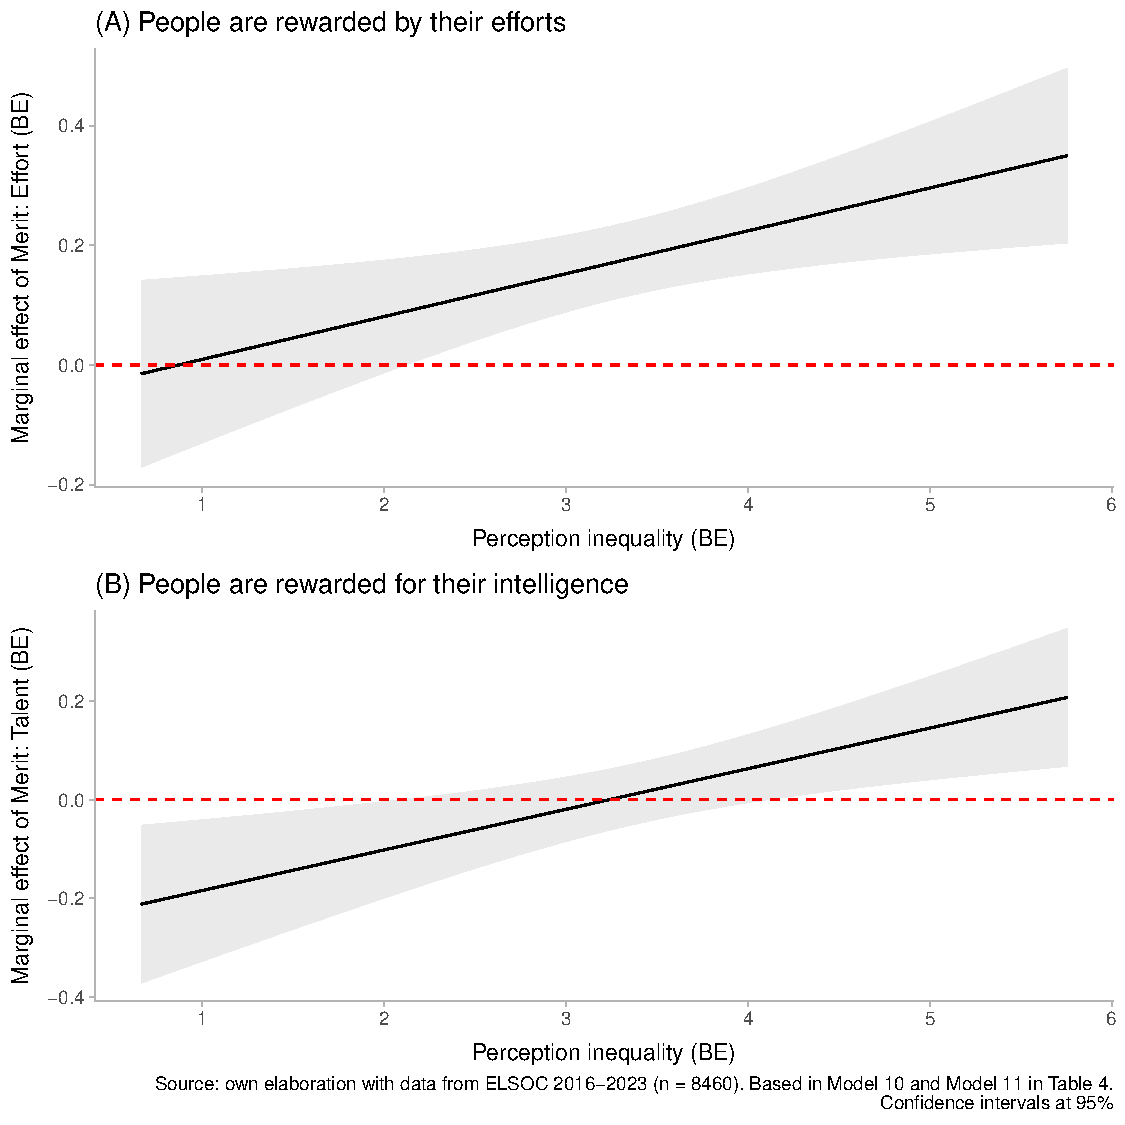
\includegraphics[width=1\textwidth,height=\textheight]{paper-blinded-resubmit_files/figure-pdf/fig-interact-1.pdf}

}

\end{figure}%

Table~\ref{tbl-interactions1} examines whether perceived economic
inequality moderates the effect of meritocratic perceptions on market
justice preferences. Contrary to our expectations, the interaction terms
in the within-person specification of Model 9 indicate that the negative
effect of talent-based meritocratic perceptions becomes stronger as
perceived inequality increases (\(\beta\) = -0.032, \(p\) \textless{}
.05). In contrast, in the between-person specification (Model 11), the
interaction term is positive (\(\beta\) = 0.099, \(p\) \textless{} .01),
suggesting that perceptions of economic inequality significantly shape
the influence of meritocratic perceptions on support for market-based
allocation of social services. Specifically, these positive effects
indicate that, as perceptions of inequality increase, the association
between talent-based meritocratic perceptions and market justice
preferences shifts in a positive direction.

The effects of effort-based meritocratic perceptions are not
statistically significant in either the within- or between-person
specifications (Models 8 and 10). However, the direction of the
coefficients is negative in the former and positive in the latter. As
shown in Figure~\ref{fig-interact}, Panel A, the between-person effect
of effort-based meritocratic perceptions on market justice preferences
strengthens as perceived inequality increases across individuals,
whereas this effect weakens among those who perceive lower levels of
inequality. Panel B reveals a similar pattern for the between-person
effect of talent-based meritocratic perceptions, although the effect is
substantially weaker at low levels of perceived inequality.

Substantively, these findings suggest that the legitimizing function of
meritocratic perceptions is amplified in contexts perceived as highly
unequal. In such contexts, meritocratic narratives may reinforce
individualistic understandings of distributive justice and intensify
support for market-based access to essential social services.

Regarding the temporal dynamics of the key predictors, the analysis
shows that time has no statistically significant effects on the
intrapersonal or interpersonal effects of perceived inequality and
meritocratic perceptions. Further details about this analysis can be
found in supplementary material.

\section{Discussion}\label{discussion}

The first set of hypotheses proposed that perceptions of economic
inequality are strongly associated with preferences for market justice.
In the between-individual specification, the effect of perceived
inequality is not statistically significant. Therefore, we cannot
conclude that individuals who, on average, perceive higher levels of
inequality are systematically less supportive of market justice. As a
result, hypothesis \(H1_{a}\) is not supported by the data. However, in
the within-individual specification, the findings reveal a significant
negative association: individuals who, at a given point in time,
perceive higher income disparities are less supportive of the idea that
access to core social services should depend on individual income. This
result aligns with theories suggesting that increased awareness of
inequality fosters a more critical stance toward market-based
distributive arrangements
(\citeproc{ref-Castillo2012a_justice}{Castillo, 2012};
\citeproc{ref-garcia-sanchez_vicious_2019}{García-Sánchez et al., 2019};
\citeproc{ref-mijs_paradox_2021}{Mijs, 2021}). Such a pattern reflects a
moral economy logic in which perceptions of systemic unfairness
undermine the legitimacy of existing distributions and strengthen
demands for greater equity. Specifically, the negative within-individual
effect over time (\(H1_{b}\)) suggests that as inequality becomes more
salient for some individuals, their support for market justice
declines---possibly due to growing distrust in market mechanisms or
increasing disillusionment with the perceived fairness of the system.

Regarding the second set of hypotheses, the results confirmed that
meritocratic perceptions---particularly those emphasizing individual
effort---were associated with stronger support for market-based
distribution systems. Individuals who believed that success is primarily
achieved through personal effort were more likely to justify unequal
access to core social services based on income, interpreting such
disparities as outcomes of individual merit rather than systemic
injustice (\(H2_{a}\)). This finding aligns with previous research
showing that meritocratic narratives serve as moral justifications that
legitimize social stratification
(\citeproc{ref-Castillo2012a_justice}{Castillo, 2012};
\citeproc{ref-hoyt_mindsets_2023}{Hoyt et al., 2023}). These perceptions
operate symbolically to reinforce structural inequalities by reducing
support for redistributive policies, framing inequality as both fair and
deserved. Consistent with prior work by Castillo et al.
(\citeproc{ref-castillo_socialization_2024}{2024}) on Chilean students,
the results suggest that such meritocratic perceptions uphold existing
hierarchies by promoting the acceptance of inequality as a reflection of
individual virtue rather than structural failure. This mechanism is
particularly salient in neoliberal contexts like Chile, where market
logics heavily shape social attitudes
(\citeproc{ref-canalesceron_sujeto_2021}{Canales Cerón et al., 2021}).

Interestingly, intra-individual changes in meritocratic perceptions over
time (\(H2_{b}\)) reveal mixed effects. While increases in the belief
that rewards are based on individual effort are associated with stronger
preferences for market justice, increases in the belief that rewards
derive from talent are linked to weaker support for such principles. One
possible explanation is that effort is generally viewed as a
controllable and malleable trait, whereas talent tends to be perceived
as innate and less subject to personal control, rendering talent-based
inequality less legitimate. Furthermore, increased exposure to
real-world scenarios in which outcomes are clearly shaped by inherent
traits rather than hard work may lead individuals to question the
fairness and legitimacy of market-based reward systems.

The third set of hypotheses addressed the moderating role of perceptions
of inequality in the relationship between meritocratic perceptions and
preferences for market justice. The analysis revealed that the positive
association between meritocratic perceptions and support for
market-based distribution systems tends to be stronger when perceived
economic inequality is high, contradicting our initial expectations
(\(H3_{a}\) and \(H3_{b}\)). Although this moderating effect is not
statistically significant for effort-related meritocratic perceptions,
it is significant for talent-related perceptions at both the within- and
between-individual levels. However, this interpretation requires
caution: the main effect of perceived inequality on support for market
justice is negative, meaning that as perceived inequality becomes less
negative (i.e., closer to zero), the positive relationship between
talent-based meritocratic perceptions and market justice preferences
becomes stronger. This suggests a more nuanced dynamic: meritocratic
perceptions, particularly those emphasizing talent, may serve as a
stronger justificatory mechanism for market-based inequalities among
individuals who are less inclined to perceive inequality as a problem.
In other words, among those who do not strongly perceive systemic
disparities, meritocratic narratives may play a more influential role in
legitimizing unequal outcomes.

Finally, the fourth exploratory hypothesis examined the potential impact
of social events --- particularly those that erupted in 2019 --- on the
relationship between meritocratic perceptions, perceptions of
inequality, and preferences for market justice. The main effect of time
indicates that, on average, support for market justice increased after
2019 protests. However, the analysis did not detect any significant
interactions between distributive beliefs and support for market
justice, suggesting that events in this period (as the mobilizations,
the pandemic and/or the constitucional processes) did not substantially
modify the underlying associations between these variables. As a result,
hypotheses \(H4_{a}\) and \(H4_{b}\) are not supported by the analysis.
This may point to a certain stability or even resilience in the
normative frameworks that guide individuals' evaluations of distributive
justice, despite the occurrence of major collective political events.
Alternatively, while the protests may have eroded trust in institutional
arrangements or governance, they may not have fundamentally altered
individuals' beliefs about how rewards and resources should be allocated
in society.

\section{Conclusions}\label{conclusions}

This study examined the complex interplay between perceptions of
economic inequality, meritocratic perceptions, and preferences toward
market justice in Chile from 2016 to 2023, drawing on longitudinal data
from the ELSOC survey. By exploring how subjective assessments and
social contexts influence support for redistribution and market-based
resource allocation, the research offers different elements that
contribute to the understanding of the normative foundations
underpinning social justice attitudes in a highly unequal and
commodified environment.

The findings support that higher perceptions of economic inequality are
associated with less support for market justice preferences, this is,
the belief that it is fair that those with higher income have better
social services such as education, pensions and health. At the same
time, meritocratic perceptions --- particularly those emphasizing
individual effort --- are strongly associated with support for
market-based distributions, suggesting that meritocracy serve as a moral
justification for structural inequalities. However, changes in
meritocratic perceptions over time reveal a more nuanced picture: while
increased emphasis on effort reinforces support for market justice,
increased emphasis on talent tends to reduce it. This distinction likely
reflects broader beliefs about the controllability and fairness of
different meritocratic traits. Moreover, the interaction between
inequality perceptions and meritocratic perceptions indicates that the
legitimizing power of meritocracy becomes stronger as perceptions of
inequality become less negative --- that is, when individuals are less
aware or concerned about economic disparities. Such finding highlights a
potential feedback mechanism by which lower sensitivity to inequality
may enable stronger endorsement of merit-based explanations for unequal
outcomes.

This research advances the extant literature by integrating subjective
perceptions with social and political contexts to explain attitudes
toward economic inequality and distributional justice. While previous
studies primarily focused on objective measures or individual
characteristics (\citeproc{ref-busemeyer_skills_2014}{Busemeyer, 2014};
\citeproc{ref-immergut_it_2020}{Immergut \& Schneider, 2020};
\citeproc{ref-lindh_public_2015}{Lindh, 2015}), this work emphasizes the
dynamic and interactional nature of perceptions and beliefs over time.
Furthermore, it highlights the importance of socio-political upheavals
in reshaping normative attitudes, underscoring the role of collective
action in challenging entrenched narratives of meritocracy and fairness.
The longitudinal approach provides a deeper temporal perspective on how
societal events could influence individual perceptions and preferences.

Regarding avenues for future research, experimental evidence could help
expand the understanding of the association between perceptual variables
and market justice preferences. International comparative studies are
also necessary in order to assess the role of national contexts and the
universality or specificity of these dynamics. Additionally,
investigating the role of media, political communication, and education
in shaping perceptions of inequality and meritocracy would deepen
understanding of the normative foundations of social justice attitudes
and their variation over time. Finally, examining how these perceptions
influence behavioral outcomes, such as political participation or
support for social movements, would provide valuable insights into the
pathways from beliefs to collective action and policy change.

\section{References}\label{references}

\phantomsection\label{refs}
\begin{CSLReferences}{1}{0}
\bibitem[\citeproctext]{ref-akyelken_urban_2020}
Akyelken, N. (2020). Urban conceptions of economic inequalities.
\emph{Regional Studies}, \emph{54}(6), 863--872.
\url{https://doi.org/10.1080/00343404.2020.1732902}

\bibitem[\citeproctext]{ref-auspurg_why_2017}
Auspurg, K., Hinz, T., \& Sauer, C. (2017). Why {Should Women Get Less}?
{Evidence} on the {Gender Pay Gap} from {Multifactorial Survey
Experiments}. \emph{American Sociological Review}, \emph{82}(1),
179--210. \url{https://doi.org/10.1177/0003122416683393}

\bibitem[\citeproctext]{ref-bates_fitting_2015}
Bates, D., Mächler, M., Bolker, B., \& Walker, S. (2015). Fitting linear
mixed-effects models using {lme4}. \emph{Journal of Statistical
Software}, \emph{67}(1), 1--48.
\url{https://doi.org/10.18637/jss.v067.i01}

\bibitem[\citeproctext]{ref-batruch_belief_2023}
Batruch, A., Jetten, J., Van De Werfhorst, H., Darnon, C., \& Butera, F.
(2023). Belief in {School Meritocracy} and the {Legitimization} of
{Social} and {Income Inequality}. \emph{Social Psychological and
Personality Science}, \emph{14}(5), 621--635.
\url{https://doi.org/10.1177/19485506221111017}

\bibitem[\citeproctext]{ref-boccardo_30_2020}
Boccardo, G. (2020). \emph{30 a{ñ}os de privatizaciones en {Chile}: {Lo}
que la pandemia revel{ó}} (Nodo XXI). Santiago.

\bibitem[\citeproctext]{ref-busemeyer_skills_2014}
Busemeyer, M. (2014). \emph{Skills and {Inequality}: {Partisan Politics}
and the {Political Economy} of {Education Reforms} in {Western Welfare
States}}. Cambridge University Press.

\bibitem[\citeproctext]{ref-busemeyer_positive_2021}
Busemeyer, M., Abrassart, A., \& Nezi, R. (2021). Beyond {Positive} and
{Negative}: {New Perspectives} on {Feedback Effects} in {Public Opinion}
on the {Welfare State}. \emph{British Journal of Political Science},
\emph{51}(1), 137--162. \url{https://doi.org/10.1017/S0007123418000534}

\bibitem[\citeproctext]{ref-canalesceron_sujeto_2021}
Canales Cerón, M., Orellana Calderón, V. S., \& Guajardo Mañán, F.
(2021). Sujeto y cotidiano en la era neoliberal: El caso de la
educaci{ó}n chilena. \emph{Revista Mexicana de Ciencias Pol{í}ticas y
Sociales}, \emph{67}(244).
\url{https://doi.org/10.22201/fcpys.2448492xe.2022.244.70386}

\bibitem[\citeproctext]{ref-castillo_cual_2009}
Castillo, J. C. (2009). {{\textquestiondown}Cu{á}l es la brecha salarial
justa? Opini{ó}n p{ú}blica y legitimaci{ó}n de la desigualdad en Chile}.
\emph{Estudios P{ú}blicos}, (113).

\bibitem[\citeproctext]{ref-Castillo2011}
Castillo, J. C. (2011). Legitimacy of {Inequality} in a {Highly Unequal
Context}: {Evidence} from the {Chilean Case}. \emph{Social Justice
Research}, \emph{24}(4), 314--340.
\url{https://doi.org/10.1007/s11211-011-0144-5}

\bibitem[\citeproctext]{ref-Castillo2012a_justice}
Castillo, J. C. (2012). Is {Inequality Becoming Just}? {Changes} in
{Public Opinion} about {Economic Distribution} in {Chile}.
\emph{Bulletin of Latin American Research}, \emph{31}(1), 1--18.
\url{https://doi.org/10.1111/j.1470-9856.2011.00605.x}

\bibitem[\citeproctext]{ref-castillo_perception_2022}
Castillo, J. C., García-Castro, J.-D., \& Venegas, M. (2022). Perception
of economic inequality: Concepts, associated factors and prospects of a
burgeoning research agenda. \emph{International Journal of Social
Psychology}, \emph{37}(1), 180--207.
\url{https://doi.org/10.1080/02134748.2021.2009275}

\bibitem[\citeproctext]{ref-castillo_multidimensional_2023}
Castillo, J. C., Iturra, J., Maldonado, L., Atria, J., \& Meneses, F.
(2023). A {Multidimensional Approach} for {Measuring Meritocratic
Beliefs}: {Advantages}, {Limitations} and {Alternatives} to the {ISSP
Social Inequality Survey}. \emph{International Journal of Sociology},
1--25. \url{https://doi.org/10.1080/00207659.2023.2274712}

\bibitem[\citeproctext]{ref-castillo_percepcion_2019}
Castillo, J. C., Miranda, D., \& Carrasco, D. (2012). Percepci{ó}n de
{Desigualdad Econ{ó}mica} en {Chile}: {Medici{ó}n}, {Diferencias} y
{Determinantes}. \emph{Psykhe (Santiago)}, \emph{21}(1), 99--114.
\url{https://doi.org/10.4067/S0718-22282012000100007}

\bibitem[\citeproctext]{ref-castillo_socialization_2024}
Castillo, J. C., Salgado, M., Carrasco, K., \& Laffert, A. (2024). The
{Socialization} of {Meritocracy} and {Market Justice Preferences} at
{School}. \emph{Societies}, \emph{14}(11), 214.
\url{https://doi.org/10.3390/soc14110214}

\bibitem[\citeproctext]{ref-chancel_world_2022}
Chancel, L., Piketty, T., Saez, E., \& Zucman, G. (2022). World
inequality report 2022.
https://bibliotecadigital.ccb.org.co/handle/11520/27510.

\bibitem[\citeproctext]{ref-davis_principles_2001}
Davis, K., \& Moore, W. E. (2001). Some {Principles} of
{Stratification}. In \emph{Social {Stratification}, {Class}, {Race}, and
{Gender} in {Sociological Perspective}, {Second Edition}} (2nd ed.).
Routledge.

\bibitem[\citeproctext]{ref-day_movin_2017}
Day, M. V., \& Fiske, S. T. (2017). Movin' on {Up}? {How Perceptions} of
{Social Mobility Affect Our Willingness} to {Defend} the {System}.
\emph{Social Psychological and Personality Science}, \emph{8}(3),
267--274. \url{https://doi.org/10.1177/1948550616678454}

\bibitem[\citeproctext]{ref-disipavlic_justification_2025}
Disi Pavlic, R., Medel, R. M., Bargsted, M., \& Somma, N. M. (2025).
Justification of violence, ideological preferences, and exposure to
protests: Causal evidence from the 2019 {Chilean} social unrest.
\emph{Social Forces}, soaf102. \url{https://doi.org/10.1093/sf/soaf102}

\bibitem[\citeproctext]{ref-dubet_repensar_2011}
Dubet, F. (2011). \emph{{Repensar la justicia social}} (Sexta
Edici{ó}n). Siglo XXI.

\bibitem[\citeproctext]{ref-easterbrook_social_2021}
Easterbrook, M. J. (2021). \emph{The social psychology of economic
inequality} (43rd ed., Vol. 2021). UNU-WIDER.
\url{https://doi.org/10.35188/UNU-WIDER/2021/981-5}

\bibitem[\citeproctext]{ref-engelhardt_what_2018}
Engelhardt, C., \& Wagener, A. (2018). What do {Germans} think and know
about income inequality? {A} survey experiment. \emph{Socio-Economic
Review}, \emph{16}(4), 743--767.
\url{https://doi.org/10.1093/ser/mwx036}

\bibitem[\citeproctext]{ref-espinoza_movilidad_2014}
Espinoza, V., \& Núñez, J. (2014). Movilidad ocupacional en {Chile}
2001-2009. {\textquestiondown}{Desigualdad} de ingresos con igualdad de
oportunidades? \emph{Revista Internacional de Sociolog{í}a},
\emph{72}(1), 57--82. \url{https://doi.org/10.3989/ris.2011.11.08}

\bibitem[\citeproctext]{ref-ferre_welfare_2023}
Ferre, J. C. (2023). Welfare regimes in twenty-first-century {Latin
America}. \emph{Journal of International and Comparative Social Policy},
\emph{39}(2), 101--127. \url{https://doi.org/10.1017/ics.2023.16}

\bibitem[\citeproctext]{ref-flores_top_2020}
Flores, I., Sanhueza, C., Atria, J., \& Mayer, R. (2020). Top {Incomes}
in {Chile}: {A Historical Perspective} on {Income Inequality},
1964--2017. \emph{Review of Income and Wealth}, \emph{66}(4), 850--874.
\url{https://doi.org/10.1111/roiw.12441}

\bibitem[\citeproctext]{ref-garcia-castro_perceiving_2020}
García-Castro, J. D., Rodríguez-Bailón, R., \& Willis, G. B. (2020).
Perceiving economic inequality in everyday life decreases tolerance to
inequality. \emph{Journal of Experimental Social Psychology}, \emph{90},
104019. \url{https://doi.org/10.1016/j.jesp.2020.104019}

\bibitem[\citeproctext]{ref-garcia-sanchez_creencias_2022}
García-Sánchez, E., \& De Carvalho, S. (2022). Las creencias que
justifican la desigualdad moderan la relaci{ó}n entre el estatus
socioecon{ó}mico y el apoyo a la redistribuci{ó}n. \emph{Revista
Internacional de Sociolog{í}a}, \emph{80}(3), e210.
\url{https://doi.org/10.3989/ris.2022.80.3.21.29}

\bibitem[\citeproctext]{ref-garcia-sanchez_attitudes_2020}
García-Sánchez, E., Osborne, D., Willis, G. B., \& Rodríguez-Bailón, R.
(2020). Attitudes towards redistribution and the interplay between
perceptions and beliefs about inequality. \emph{British Journal of
Social Psychology}, \emph{59}(1), 111--136.
\url{https://doi.org/10.1111/bjso.12326}

\bibitem[\citeproctext]{ref-garcia-sanchez_vicious_2019}
García-Sánchez, E., Van Der Toorn, J., Rodríguez-Bailón, R., \& Willis,
G. B. (2019). The {Vicious Cycle} of {Economic Inequality}: {The Role}
of {Ideology} in {Shaping} the {Relationship Between} {``{What Is}''}
and {``{What Ought} to {Be}''} in 41 {Countries}. \emph{Social
Psychological and Personality Science}, \emph{10}(8), 991--1001.
\url{https://doi.org/10.1177/1948550618811500}

\bibitem[\citeproctext]{ref-garcia-sanchez_perceptions_2018}
García-Sánchez, E., Willis, G. B., Rodríguez-Bailón, R., Palacio Sañudo,
J., David Polo, J., \& Rentería Pérez, E. (2018). Perceptions of
{Economic Inequality} and {Support} for {Redistribution}: {The} role of
{Existential} and {Utopian Standards}. \emph{Social Justice Research},
\emph{31}(4), 335--354. \url{https://doi.org/10.1007/s11211-018-0317-6}

\bibitem[\citeproctext]{ref-gijsberts_thelegitimation_1999}
Gijsberts, M. (1999). \emph{{Thelegitimation of inequality in state-
socialist and market societies, 1987 - 1996}}. Amsterdam: Thela Thesis.

\bibitem[\citeproctext]{ref-gimpelson_misperceiving_2018}
Gimpelson, V., \& Treisman, D. (2018). Misperceiving inequality.
\emph{Economics \& Politics}, \emph{30}(1), 27--54.
\url{https://doi.org/10.1111/ecpo.12103}

\bibitem[\citeproctext]{ref-hadler_why_2005}
Hadler, M. (2005). Why {Do People Accept Different Income Ratios}?: {A
Multi-level Comparison} of {Thirty Countries}. \emph{Acta Sociologica},
\emph{48}(2), 131--154. \url{https://doi.org/10.1177/0001699305053768}

\bibitem[\citeproctext]{ref-hauser_misperceptions_2017}
Hauser, O. P., \& Norton, M. I. (2017). ({Mis})perceptions of
inequality. \emph{Current Opinion in Psychology}, \emph{18}, 21--25.
\url{https://doi.org/10.1016/j.copsyc.2017.07.024}

\bibitem[\citeproctext]{ref-hoxMultilevelAnalysisTechniques2017a}
Hox, J. J., Moerbeek, M., \& Van de Schoot, R. (2017). \emph{Multilevel
{Analysis}: {Techniques} and {Applications}}.

\bibitem[\citeproctext]{ref-hoyt_mindsets_2023}
Hoyt, C. L., Burnette, J. L., Billingsley, J., Becker, W., \& Babij, A.
D. (2023). Mindsets of poverty: {Implications} for redistributive policy
support. \emph{Analyses of Social Issues and Public Policy},
\emph{23}(3), 668--693. \url{https://doi.org/10.1111/asap.12367}

\bibitem[\citeproctext]{ref-immergut_it_2020}
Immergut, E. M., \& Schneider, S. M. (2020). Is it unfair for the
affluent to be able to purchase {``better''} healthcare? {Existential}
standards and institutional norms in healthcare attitudes across 28
countries. \emph{Social Science \& Medicine}, \emph{267}, 113146.
\url{https://doi.org/10.1016/j.socscimed.2020.113146}

\bibitem[\citeproctext]{ref-janmaat_subjective_2013}
Janmaat, J. G. (2013). Subjective inequality: {A} review of
international comparative studies on people's views about inequality.
\emph{Archives Europeennes de Sociologie}, \emph{54}(3), 357--389.
\url{https://doi.org/10.1017/S0003975613000209}

\bibitem[\citeproctext]{ref-kluegel_social_1995a}
Kluegel, J. R., Mason, D. S., \& Wegener, B. (Eds.). (1995).
\emph{Social {Justice} and {Political Change}: {Public Opinion} in
{Capitalist} and {Post-Communist States}} (1st ed.). Routledge.

\bibitem[\citeproctext]{ref-kluegel_legitimation_1999}
Kluegel, J. R., Mason, D. S., \& Wegener, B. (1999). The {Legitimation}
of {Capitalism} in the {Postcommunist Transition}: {Public Opinion}
about {Market Justice}, 1991-1996. \emph{European Sociological Review},
\emph{15}(3), 251--283. Retrieved from
\url{https://www.jstor.org/stable/522731}

\bibitem[\citeproctext]{ref-kluegel_beliefs_1981}
Kluegel, J. R., \& Smith, E. R. (1981). Beliefs {About Stratification}.
\emph{Annual Review of Sociology}, 29--56.

\bibitem[\citeproctext]{ref-kluegel_beliefs_1986}
Kluegel, J. R., \& Smith, E. R. (1986). \emph{Beliefs about
{Inequality}: {Americans}' {Views} of {What Is} and {What Ought} to
{Be}} (1st ed.). Routledge.

\bibitem[\citeproctext]{ref-koos_moral_2019}
Koos, S., \& Sachweh, P. (2019). The moral economies of market
societies: Popular attitudes towards market competition, redistribution
and reciprocity in comparative perspective. \emph{Socio-Economic
Review}, \emph{17}(4), 793--821.
\url{https://doi.org/10.1093/ser/mwx045}

\bibitem[\citeproctext]{ref-kuhn_eye_2011}
Kuhn, A. (2011). In the eye of the beholder: {Subjective} inequality
measures and individuals' assessment of market justice. \emph{European
Journal of Political Economy}, \emph{27}(4), 625--641.
\url{https://doi.org/10.1016/j.ejpoleco.2011.06.002}

\bibitem[\citeproctext]{ref-lane_political_1962}
Lane, R. (1962). \emph{Political ideology: Why the {American} common man
believes what he does}. Oxford, England: Free Press of Glencoe.

\bibitem[\citeproctext]{ref-lane_market_1986}
Lane, R. (1986). Market {Justice}, {Political Justice}. \emph{American
Political Science Review}, \emph{80}(2), 383--402.
\url{https://doi.org/10.2307/1958264}

\bibitem[\citeproctext]{ref-lee_fairness_2023}
Lee, J.-S., \& Stacey, M. (2023). Fairness perceptions of educational
inequality: The effects of self-interest and neoliberal orientations.
\emph{The Australian Educational Researcher}.
\url{https://doi.org/10.1007/s13384-023-00636-6}

\bibitem[\citeproctext]{ref-lindh_public_2015}
Lindh, A. (2015). Public {Opinion} against {Markets}? {Attitudes}
towards {Market Distribution} of {Social Services} -- {A Comparison} of
17 {Countries}. \emph{Social Policy \& Administration}, \emph{49}(7),
887--910. \url{https://doi.org/10.1111/spol.12105}

\bibitem[\citeproctext]{ref-lindh_bringing_2023}
Lindh, A., \& McCall, L. (2023). Bringing the market in: An expanded
framework for understanding popular responses to economic inequality.
\emph{Socio-Economic Review}, \emph{21}(2), 1035--1055.
\url{https://doi.org/10.1093/ser/mwac018}

\bibitem[\citeproctext]{ref-lopez-roldan_comparative_2021}
López-Roldán, P., \& Fachelli, S. (Eds.). (2021). \emph{Towards a
{Comparative Analysis} of {Social Inequalities} between {Europe} and
{Latin America}}. Cham: Springer International Publishing.
\url{https://doi.org/10.1007/978-3-030-48442-2}

\bibitem[\citeproctext]{ref-mac-clure_justicia_2024}
Mac-Clure, O., Barozet, E., \& Franetovic, G. (2024). {Justicia
distributiva y posici{ó}n social subjetiva: {\textquestiondown}la
meritocracia justifica la desigualdad de ingresos?} \emph{Convergencia
Revista de Ciencias Sociales}, \emph{31}, 1.
\url{https://doi.org/10.29101/crcs.v31i0.22258}

\bibitem[\citeproctext]{ref-madariaga_three_2020}
Madariaga, A. (2020). The three pillars of neoliberalism: {Chile}'s
economic policy trajectory in comparative perspective.
\emph{Contemporary Politics}, \emph{26}(3), 308--329.
\url{https://doi.org/10.1080/13569775.2020.1735021}

\bibitem[\citeproctext]{ref-mccall_exposure_2017}
McCall, L., Burk, D., Laperrière, M., \& Richeson, J. A. (2017).
Exposure to rising inequality shapes {Americans}' opportunity beliefs
and policy support. \emph{Proceedings of the National Academy of
Sciences}, \emph{114}(36), 9593--9598.
\url{https://doi.org/10.1073/pnas.1706253114}

\bibitem[\citeproctext]{ref-mijs_stratified_2016}
Mijs, J. (2016a). Stratified {Failure}: {Educational Stratification} and
{Students}' {Attributions} of {Their Mathematics Performance} in 24
{Countries}. \emph{Sociology of Education}, \emph{89}(2), 137--153.
\url{https://doi.org/10.1177/0038040716636434}

\bibitem[\citeproctext]{ref-mijs_unfulfillable_2016}
Mijs, J. (2016b). The {Unfulfillable Promise} of {Meritocracy}: {Three
Lessons} and {Their Implications} for {Justice} in {Education}.
\emph{Social Justice Research}, \emph{29}(1), 14--34.
\url{https://doi.org/10.1007/s11211-014-0228-0}

\bibitem[\citeproctext]{ref-mijs_paradox_2021}
Mijs, J. (2021). The paradox of inequality: Income inequality and belief
in meritocracy go hand in hand. \emph{Socio-Economic Review},
\emph{19}(1), 7--35. \url{https://doi.org/10.1093/ser/mwy051}

\bibitem[\citeproctext]{ref-mijs_belief_2022}
Mijs, J., Daenekindt, S., de Koster, W., \& van der Waal, J. (2022).
Belief in {Meritocracy Reexamined}: {Scrutinizing} the {Role} of
{Subjective Social Mobility}. \emph{Social Psychology Quarterly},
\emph{85}(2), 131--141. \url{https://doi.org/10.1177/01902725211063818}

\bibitem[\citeproctext]{ref-pedersen_attitudes_2019}
Pedersen, R. T., \& Mutz, D. C. (2019). Attitudes {Toward Economic
Inequality}: {The Illusory Agreement}. \emph{Political Science Research
and Methods}, \emph{7}(04), 835--851.
\url{https://doi.org/10.1017/psrm.2018.18}

\bibitem[\citeproctext]{ref-pierson_when_1993}
Pierson, P. (1993). When {Effect Becomes Cause}: {Policy Feedback} and
{Political Change}. \emph{World Politics}, \emph{45}(4), 595--628.
\url{https://doi.org/10.2307/2950710}

\bibitem[\citeproctext]{ref-reynolds_perceptions_2014}
Reynolds, J., \& Xian, H. (2014). Perceptions of meritocracy in the land
of opportunity. \emph{Research in Social Stratification and Mobility},
\emph{36}, 121--137. \url{https://doi.org/10.1016/j.rssm.2014.03.001}

\bibitem[\citeproctext]{ref-sandel_tyranny_2020}
Sandel, M. J. (2020). \emph{The tyranny of merit: {What}'s become of the
common good?} (First edition). New York: {Farrar, Straus and Giroux}.

\bibitem[\citeproctext]{ref-schneider_poverty_2015}
Schneider, S. M., \& Castillo, J. C. (2015). Poverty {Attributions} and
the {Perceived Justice} of {Income Inequality} : {A Comparison} of
{East} and {West Germany}.
\url{https://doi.org/10.1177/0190272515589298}

\bibitem[\citeproctext]{ref-schroder_income_2017}
Schröder, M. (2017). Is {Income Inequality Related} to {Tolerance} for
{Inequality}? \emph{Social Justice Research}, \emph{30}(1), 23--47.
\url{https://doi.org/10.1007/s11211-016-0276-8}

\bibitem[\citeproctext]{ref-singer_applied_2009}
Singer, J. D., \& Willett, J. B. (2009). \emph{Applied longitudinal data
analysis: Modeling change and event occurence}. New York: Oxford
University Press, Incorporated.

\bibitem[\citeproctext]{ref-somma_no_2021}
Somma, N. M., Bargsted, M., Disi Pavlic, R., \& Medel, R. M. (2021). No
water in the oasis: The {Chilean Spring} of 2019--2020. \emph{Social
Movement Studies}, \emph{20}(4), 495--502.
\url{https://doi.org/10.1080/14742837.2020.1727737}

\bibitem[\citeproctext]{ref-svallfors_political_2007}
Svallfors, S. (Ed.). (2007). \emph{The {Political Sociology} of the
{Welfare State}: {Institutions}, {Social Cleavages}, and {Orientations}}
(1st ed.). Stanford University Press.
\url{https://doi.org/10.2307/j.ctvr0qv0q}

\bibitem[\citeproctext]{ref-tejero-peregrina_perceived_2025}
Tejero-Peregrina, L., Willis, G., Sánchez-Rodríguez, Á., \&
Rodríguez-Bailón, R. (2025). From {Perceived Economic Inequality} to
{Support} for {Redistribution}: {The Role} of {Meritocracy Perception}.
\emph{International Review of Social Psychology}, \emph{38}(1), 4.
\url{https://doi.org/10.5334/irsp.1013}

\bibitem[\citeproctext]{ref-torche_intergenerational_2014a}
Torche, F. (2014). Intergenerational {Mobility} and {Inequality}: {The
Latin American Case}. \emph{Annual Review of Sociology}, \emph{40}(1),
619--642. \url{https://doi.org/10.1146/annurev-soc-071811-145521}

\bibitem[\citeproctext]{ref-trump_income_2018}
Trump, K.-S. (2018). Income {Inequality Influences Perceptions} of
{Legitimate Income Differences}. \emph{British Journal of Political
Science}, \emph{48}(4), 929--952.
\url{https://doi.org/10.1017/S0007123416000326}

\bibitem[\citeproctext]{ref-vondemknesebeck_are_2016}
Von Dem Knesebeck, O., Vonneilich, N., \& Kim, T. J. (2016). Are health
care inequalities unfair? {A} study on public attitudes in 23 countries.
\emph{International Journal for Equity in Health}, \emph{15}(1), 61.
\url{https://doi.org/10.1186/s12939-016-0350-8}

\bibitem[\citeproctext]{ref-willis_legitimacy_2015}
Willis, G. B., Rodríguez-Bailón, R., López-Rodríguez, L., \&
García-Sánchez, E. (2015). Legitimacy {Moderates} the {Relation Between
Perceived} and {Ideal Economic Inequalities}. \emph{Social Justice
Research}, \emph{28}(4), 493--508.
\url{https://doi.org/10.1007/s11211-015-0253-7}

\bibitem[\citeproctext]{ref-wilson_role_2003}
Wilson, C. (2003). The {Role} of a {Merit Principle} in {Distributive
Justice}. \emph{The Journal of Ethics}, \emph{7}(3), 277--314.
\url{https://doi.org/10.1023/A:1024667228488}

\bibitem[\citeproctext]{ref-young_rise_1962}
Young, M. (1962). \emph{The rise of the meritocracy}. Baltimore: Penguin
Books.

\end{CSLReferences}



\end{document}
